\documentclass[11pt,twoside,a4paper]{report}

\usepackage[utf8]{inputenc}
\usepackage[T1]{fontenc}


\usepackage{amsmath,amsfonts,amssymb}
\usepackage{graphicx}
\usepackage{float}
\usepackage[lined,boxed,commentsnumbered]{algorithm2e}

\usepackage[usenames, dvipsnames]{color}
\usepackage{fancyhdr}
\usepackage[toc,page]{appendix}
\usepackage{subfig}


\title{A super cool scientific Title ...}
\author{Gautier VAILLANT}

\fancypagestyle{newstyle}{
\fancyhf{} % clear all header and footer fields
\fancyhead[l]{\bfseries \nouppercase \rightmark} % except the center
\fancyfoot[R]{\thepage} % except the center
\renewcommand{\headrulewidth}{0pt}
\renewcommand{\footrulewidth}{0pt}}

\pagestyle{newstyle}

\usepackage{listings}
\usepackage{color}

\definecolor{dkgreen}{rgb}{0,0.6,0}
\definecolor{gray}{rgb}{0.5,0.5,0.5}
\definecolor{mauve}{rgb}{0.58,0,0.82}

\lstset{frame=tb,
  language=C++,
  aboveskip=3mm,
  belowskip=3mm,
  showstringspaces=false,
  columns=flexible,
  basicstyle={\small\ttfamily},
  numbers=none,
  numberstyle=\tiny\color{gray},
  keywordstyle=\color{blue},
  commentstyle=\color{dkgreen},
  stringstyle=\color{mauve},
  breaklines=true,
  breakatwhitespace=true,
  tabsize=3
}

\setcounter{tocdepth}{4}

\begin{document}

\maketitle



\chapter*{Abstract}

Simulating systems with long-range pairwise interactions is a frequently encountered challenge in scientific research.It plays an important role in Astrophysics to know the dynamics of galaxies, in plasma physics or in our case in biophysics.  A direct evaluation of these pairwise interactions leads to $\mathcal{O}(N^2)$, which obviously scaled badly with a system of size $N$. 
Some other techniques, such as the PME (Particle Mesh Ewald) and the FMM (Fast Multipole Method) obtain a complexity of $\mathcal{O}(N\log(N))$ and $\mathcal{O}(N)$,  respectively these techniques also allow a greater scalability of the system for parallel computations.

The aim of this internship is to study how the FMM compares to the PME, ie. which sets of parameters gives the same accuracy  for both methods. We developed some tools to compare the data from softwares simulating systems for both methods and study their accuracy. 
\\
\\
\\

La simulation de systèmes avec des interactions a longues distances est un problème très fréquemment rencontre dans la recherche scientifique. Elles jouent un rôle important en physique pour connaître la dynamique des galaxies, en physique des plasmas ou encore dans notre cas en biophysique. L'évaluation directe de ces interactions nous amène a une complexité en $\mathcal{O}(N^2)$, qui supporte difficilement la mise a l'échelle : De plus il est impossible avec cette méthode de pouvoir simuler un système infini.
	Certaines techniques, telles que la PME (Particle Mesh Ewald) et la FMM (Fast Multipole Method) ont une complexité respectivement de $\mathcal{O}(N\log(N))$ et $\mathcal{O}(N)$ . Elles permettent de pouvoir gérer des systèmes avec conditions aux limites périodiques ; elles supportent aussi bien mieux la mise a l'échelle pour le calcul parallèle.
	
	Le but de ce stage est d'etudier comment la FMM peut ete comparee a la PME, c'est a dire quels ensemble de parameteres nous donne la meme precision four les deux methodes.


\chapter*{Acknowledgments}

I would first like to gratefully thank Helmut Grubmüller and Bert de Groot for welcoming me in their lab. I also thank Carsten Kutzner who supervised my Internship. I also would like to Thank Bartosz Kohnke and Thomas Ullmann for providing me advice on my project.\\ 

Finally I would also like to thank Ivo Kabadschow and Andreas Beckmann who welcomed me in the Jülich Forschungszentrum to teach me the details of the FMM method. 

\tableofcontents
\listoffigures

\chapter{Presentation of the Lab}
\section*{Max Planck Institute for Biophysical Chemistry}

The Max Planck Institute for Biophysical Chemistry is part of the Max Planck Institutes, which are an ensemble of research center throughout Germany (As the CNRS in France could be).\\

The Max-Planck Institute for Biophysical Chemistry, located in Göttingen, is one of the biggest research centers in the Biophysics field in Europe. Its research fields includes Molecular Dynamics Simulation, but also NMR or Biochemistry.\\
The departments are : (from http://www.mpibpc.mpg.de/groups)
\begin{itemize}
\item Patrick Cramer - Molecular Biology
\item Gregor Eichele – Genes and Behavior
\item Dirk Görlich – Cellular Logistics
\item Christian Griesinger – NMR-based Structural  Biology
\item \textbf{Helmut Grubmüller – Theoretical and Computational Biophysics}
\item Stefan W. Hell – NanoBiophotonics
\item Herbert Jäckle – Molecular Developmental Biology
\item Reinhard Jahn – Neurobiology
\item Reinhard Lührmann – Cellular Biochemistry
\item Marina V. Rodnina – Physical Biochemistry
\item Melina Schuh – Meiosis 
\item Alec M. Wodtke – Dynamics at Surfaces
\end{itemize}

\section*{Department of Theoretical and Computational Biophysics}

This department is led by Helmut Grubmüller. It aims at understanding of the physics and function of proteins, protein complexes, and other biomolecular structures at the atomic level. For this purpose, dynamic complex atomisitic computer simulations are carried out.\\

One area of research is on studying systems (Proteins, membranes) and molecular machines in order to better understand their dynamics (for example the molecular mechanisms of the ribosome), and another area is focusing on method development.
Concerning the part of the department dedicated to methods and theory, new statistical mechanics concepts, quantum hybrid methods, and efficient parallel simulation algorithms and codes are the methodological focus of the department.

Both lines of questions phrased above are closely interlinked. Progress in the understanding of the physics of proteins, on the one hand, enables improved and more realistic simulation techniques, which allow to study a growing number of biochemical processes in great detail. Through analysis of well-understood mechanisms, on the other hand, one can learn to separate relevant aspects in protein dynamics from irrelevant ones — which is prerequisite for the construction of effective protein models. In short, we find a close interplay between method development, algorithmic progress, and application.  






\chapter{Context of the Internship}

The context of this internship is driven by the "SPPEXA (Software for exascale computing) / GromEx" project funded by the DFG (Deutsche Forschungsgemeinschaft).
The Idea of this project is to create a flexible and fast solver for computing forces and potentials, which is a preliminary for molecular simulations.

A poster\footnote{from http://www.mpibpc.mpg.de/grubmueller/sppexa}   of the project can be found below :

\begin{figure}[H]

\includegraphics[scale=2]{sppexa-poster}
 \centering 
\caption{Poster for the SPEXXA project}
\label{fig:poster}
\end{figure}


The currently established method for computing electrostatic forces is the PME (Particle Mesh Ewald) \cite{darden1993particle}. One of its problems is a communication bottleneck that prohibits efficient parallelization across many (> 10000) CPU cores. The idea would be to replace this method with a new method called the Fast-Multipole (FMM) Method which is based on a tree structure and may allow an greater parallelization of the system as wanted.\\

So the idea of the internship is first to know how to tune those systems to know how they relate to each other. Both PME and FMM make approximations. For a fair comparison we want to compare the methods at equal accuracy of the forces (and energies) they compute. 

\chapter{Methods for computing electrostatic forces}

The electrostatic potential of a group of $N$ of charge $q_i$ at position $r_i$ is defined as :

\begin{equation}
V_C = \frac{1}{4\pi\epsilon_0} \sum\limits_{i=1}^{N}\sum\limits_{j>i} \frac{q_i q_j}{r_{ij}}
\end{equation}

Computing this potential is very important in different areas of physics, such as plasma physics, or in our case molecular dynamics where the forces between charged particles need to be computed in an efficient and scalable way, the force being computed using

\begin{equation}
	\vec{F}_i = - \vec{\nabla_i} V(\vec{r})
\end{equation}


\section{Direct summation method }


In this section, we will explain the most basic method to compute pairwise interactions and explain why the method leads to long computation times and sometimes .

\subsection{"Naive" $\mathcal{O}(N^2)$ Method}

The sum of all electrostatic forces $F_i$ exerted  on one particle can be written the following way:

\begin{equation}
	F_i =  \sum\limits_{i=1}^{N}\sum\limits_{j>i} \frac{q_i q_j}{4\pi\epsilon_0 r_{ij^2}}
	\label{coulombComplete}
\end{equation}

where $q$ is the charge of one particle, and $r_{ij}$ is the distance between particle $i$ and particle $j$.

In the thesis we will simplify the equation ~\eqref{coulombComplete} by just writing:

\begin{equation}
	\vec{F}_i =  f\cdot\sum\limits_{i=1}^{N}\sum\limits_{j>i} \frac{q_i q_j}{r_{ij^2}} \frac{\vec{r_{ij}}}{|r_{ij}|}
	\label{coulombSimplified}
\end{equation}

where $f=\frac{1}{4\pi\epsilon_0}$ is called the \textbf{electric conversion factor} and is equal to 138.935485(9) kJ.mol$^-1$.nm.e$^{-2}$\\


The first, naive way to compute electrostatic forces is just to follow equation (\ref{coulombSimplified}):

So if we consider a set of $N$ charged particles, $N-1$ interactions are needed to compute the force acting on one specific particle. So in order to know the forces of the set of particles, $N\cdot(N-1)$ operations are needed, hence an algorithmic complexity of $\mathcal{O}(N^2)$. Indeed, in order to have to have a physically accurate simulation, it is need to surround the molecule we want to study into a solvent (often water) : If the layer of water is finite, it can lead to some unexpected effects as shown [REF...]\\

This gives the following algorithm:

\IncMargin{1em}
\begin{algorithm}[H]

\SetKwData{Left}{left}\SetKwData{This}{this}\SetKwData{Up}{up}
\SetKwData{Force}{force}

\SetKwFunction{ComputeForce}{computeForce}
\SetKwFunction{Union}{Union}\SetKwFunction{FindCompress}{FindCompress}
\SetKwInOut{Input}{input}\SetKwInOut{Output}{output}

\Input{A set of $N$ charged particles}
\Output{A list of the forces
for each particle}
\BlankLine

\emph{For each particle i}\;
\For{$i\leftarrow 1$ \KwTo $N-1$}{
\emph{add interaction between particle $i$ and particle $j$ }\;
\For{$j\leftarrow i+1$ \KwTo $N$}{

	\Force$[i]$  $\leftarrow$ \Force$[i]$ + \ComputeForce{$i,j$}   \;

}
}
\caption{Naive method}\label{algo_disjdecomp}
\end{algorithm}\DecMargin{1em}


The complexity of such a computation limits its use to rather small systems and is not really usable for bigger systems such as proteins or astrophysical systems.
 Moreover it is also important to say that if we want to add periodic boundary conditions the $\mathcal{O}(N^2)$ method is not usable as the system is infinite.


\subsection{Possible improvements}

A possible method to overcome this limitation for periodic systems is to limit the interaction to a certain radius : if the distance between two particles if greater than $R_0$, then the force is set to $0$.

So we have the following system :


\begin{equation}
  \overrightarrow{F}_{A \rightarrow B}  =
	\begin{cases}
	  \frac{q_A q_B \vec{r}_{AB} }{|R_{AB}|^2}  & \text{if } R_{AB} < R_0 \\
	  \overrightarrow{0} & \text{otherwise}
	\end{cases}
\end{equation}

This technique is for example used for Lennard-Jones potentials ($V_{LJ} = 4\epsilon [(\frac{\sigma}{r})^12 - (\frac{\sigma}{r})^6] $), where the intensity of the force is quickly decreasing. It allows to limit the number of interactions to only the close neighbors.\\

However, one of the problems of this cutoff technique, especially for long-range interactions such as coulombic interactions using a cut-off can lead to artifacts resulting from the sudden drop of the force to 0 at the cutoff. It was shown that this can lead to unphysical assemblies of particles at the cutoff distance as shown for instance in figure (\ref{fig:artefact}) .

\begin{figure}[H]

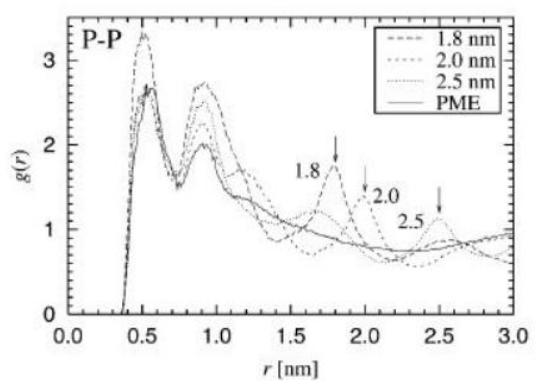
\includegraphics[scale=0.8]{artefact}
 \centering
 
\caption{Radial distribution function (RDF) $g(r)$ between the two
central atoms in the head-group of lipids: Cutoff distances are indicated by arrows. From \cite{patra2003molecular}  }

\label{fig:artefact}

\end{figure}


As we can see in figure \ref{fig:artefact},  the radial distribution of the distance between two atom shows a peak, corresponding to the cutoff of the system. This shows that by using a cutoff technique we might see some artifacts.\\

So we can see at least three reasons not to use the direct summation method : The first and main reason is that the method doesn't work with periodic boundary conditions. Then, is cutoff methods are used to solve the problem, artifacts might arise at cutoff distances. Finally the method is computationally inefficient.



%-------------------------------------------------------------------------------------------


\section{Fourier Transform-Based methods}

To compute the potentials and the forces of particles,  Fourier-transform based techniques have been developed in order to overcome the problems stated above .

\subsection{Ewald Summation}

This subset of techniques comes from a theoretical physics technique called the Ewald summation.

in periodic boundary conditions, the Coulomb potential $V_C$ is:

\begin{equation}
	V = \sum_{n_x,n_y,n_z} \sum_{i}^{N} \sum_{j>i} \frac{q_i q_j}{r_{ij}}
	\label{periodicSum}
\end{equation}
where $n_x,n_y,n_z$ are the box index vector.\\

The equation (\ref{periodicSum}) is conditionally convergent and slow to converge. One technique discovered by Ewald is to split the potential in two absolutely convergent terms and one constant term:


$\frac{1}{r}$ can be written in the following way :

\begin{equation}
   \frac{1}{r} = \frac{f(x)}{r} + \frac{1 - f(x)}{r}
\end{equation}

The idea is to choose $f$, so that $\frac{f(x)}{r}$ is quickly decaying and can be computed in real space with a cutoff at high accuracy. At the same time, we want $\frac{1 - f(x)}{r}$ is as smooth as possible and therefore be represented in reciprocal sapce with just a few $\vec{k}$ vectors This gives a quick and accurate computation of the real and the reciprocal space where $V = V_{\text{direct}} + V_{\text{reciprocal}}$\\

A good choice is often $f(x) = \text{erfc}(\alpha x)$,the complementary error function, where $\alpha$ is called the splitting parameter, and $\text{erfc}(x) = \frac{2}{\sqrt{\pi}} \int_{x}^{+\infty}{e^{-t^2}\text{dt}} $\\

so we obtain the following potentials :\\

For the direct space :

\begin{equation}
   V_{\text{direct}} =  \frac{1}{2} \sum_{\vec{n}} \sum_{i,j}^{N} q_i q_j \frac{\text{erfc}(\alpha r)}{r}
\end{equation}

and for the reciprocal space :

\begin{equation}
\label{Vrecip}
	V_{\text{reciprocal}} = \frac{1}{2 \pi L} \sum_{i,j}^{N} q_i q_j \sum_{\vec{m}}\frac{\exp{-(\pi \overrightarrow{m}/\alpha)^2} +2\pi i \overrightarrow{m} \cdot (r_i - r_j)}{\overrightarrow{m}^2}
\end{equation}

where $\vec{m}$ are the vectors in the reciprocal space, and $L$ is the volume of the cell.\\

\begin{equation*}
\hspace{10 mm}
\left\lbrace
\begin{array}{ccc}
\vec{m}_x = & 2\pi \frac{\vec{n_y}\times\vec{n_z}}   {\vec{n_x}\cdot(\vec{n_y}\times\vec{n_z})} + n\cdot L_x        \\
\vec{m}_y = &  2\pi \frac{\vec{n_z}\times\vec{n_x}}   {\vec{n_y}\cdot(\vec{n_z}\times\vec{n_x})} + n\cdot L_y \\
\vec{m}_z = & 2\pi \frac{\vec{n_x}\times\vec{n_y}}   {\vec{n_x}\cdot(\vec{n_z}\times\vec{n_y})} + n\cdot L_z  
\end{array}\right.
, n \in \mathbb{Z}
\end{equation*}


Once the electrostatic potentials are obtained, it is possible to differentiate the potentials with respect to the position $p=(x,y,z)$ to obtain the force on each particle.\\

\begin{equation}
   \overrightarrow{F}_i^{\text{direct}} = \overrightarrow{\nabla}_i V_{\text{direct}} 
\end{equation}


so we have:

\begin{equation}
\label{ewaldDirect}
   \overrightarrow{F}_p^{\text{direct}} = q_i \sum\limits_{i=1,i\neq j}^N \sum\limits_{\vec{n}} q_j \frac{(r_{ij,\vec{n}})_p}{r_{ij,\vec{n}}^3}
   \{\text{erfc}(\alpha (r_{ij,\vec{n}}) + \frac{2\alpha}{\sqrt{\pi}} r_{ij,\vec{n}} \exp(-(\alpha r_{ij,\vec{n}})^2)\}
\end{equation}


\begin{equation}
\label{ewaldReciprocal}
   \overrightarrow{F}_p^{\text{reciprocal}} = \frac{2 q_i}{L} \sum\limits_{i=1,i\neq j}^N \sum_{\vec{m} \neq 0} \frac{\vec{m}_p^*}{\vec{m}^{*^2}} \exp{(-(\frac{\pi \vec{m}}{\alpha L})^2)}\sin{\frac{2\pi}{L} m \cdot r_{ij} }
\end{equation}

Equations \ref{ewaldDirect} and \ref{ewaldReciprocal} can then be used to compute the force on each particle by adding the direct space and the reciprocal space contribution.\\


\subsection{PME}
One way to improve this method is to compute the Fourier sum using the FFT (Fast Fourier Transform). This allows the algorithm to get a complexity of $\mathcal{O}(N\log N)$. There is different methods that are based on the Ewald summation, namely the \textbf{P3M} (Particle-Particle Particle-Mesh Method) or the \textbf{FFP} (Fast Fourier Poisson method). Descriptions of these methods can be found \cite{toukmaji1996ewald}. 

In our case, we will focus on the \textbf{PME} method as it is the method currently used in GROMACS. \\

We remind that the potential for the reciprocal space $V_{\text{reciprocal}}$ is written in equation (\ref{Vrecip}):


\begin{equation*}
    V_{\text{reciprocal}} =\frac{1}{2 \pi V} \sum\limits_{i,j}^{N} q_i q_j \sum\limits_{\textbf{n}^*} \frac{\exp{(-(\pi \overrightarrow{m}/\alpha)^2} +2\pi i \overrightarrow{m} \cdot (r_i - r_j))}{m^2}    
\end{equation*}



This equation can be rewritten as :

\begin{equation*}
    V_{\text{reciprocal}} =\frac{1}{2 \pi V} \sum\limits_{\textbf{n}^* \neq 0}^{N}  \frac{\exp{-(\pi \overrightarrow{m}/\alpha)^2}}{\overrightarrow{m}^2}S(-\overrightarrow{m} )S(\overrightarrow{m} )
\end{equation*}

where $S(\textbf{n}^* )$ is defined as the Structure factor:

\begin{equation}
    S(\textbf{n}^* ) = \sum\limits_{k=1}^{N} {q_k \exp(2 \pi i \vec{m} \cdot \textbf{r}) }
\end{equation}


The idea of the PME is to approximate the structure factor $S(\vec{m})$ by the 3D Fourier Transform of the charge matrix,which is obtained by interpolating the charges to a discrete grid of size $ p_x \times p_y \times p_z $. 
	Let also define $\mathcal{F}(Q)$ the 3D FFT of $Q$. The charges $q_i$ are mapped to the grid using interpolation.Originally, Lagrange interpolation was used, but now a b-spline interpolation is used. The order of interpolation is called the \textit{PME Order}\\

then the Structure factor can be approximated as its FFT :

\begin{equation}
   S(\overrightarrow{m}) \approx \widetilde{S}(\overrightarrow{m}) = \mathcal{F}(Q)(\overrightarrow{m})
\end{equation}

so the reciprocal energy can also be approximated by:

\begin{equation}
   V_{\text{reciprocal}} \approx \widetilde{V}_{\text{reciprocal}}   =\frac{1}{2 \pi V} \sum\limits_{\textbf{n}^* \neq 0}^{N}  \frac{\exp{(-(\pi \overrightarrow{m}/\alpha)^2)}}{m^2}\mathcal{F}(Q)(\textbf{m})\mathcal{F}(Q)(-\textbf{m})
\end{equation} \\

It can be shown that the complexity of such a system is $\mathcal{O}(N \log(N))$ which is a much bigger improvement compared to the $\mathcal{O}(N^2)$ complexity of the direct algorithm. Then it also allows to handle infinite systems with periodic boundary conditions.\\ However, the algorithm doesn't scale well for large scale parallelism (above 10000 CPU cores)\cite{kutzner2013scaling}. The bottleneck is located in the computation of the FFT, where an all-to-all communication is required, hence the need for a more scalable algorithm for the computations of electrostatic forces as shown \cite{kutzner2013scaling}.

\begin{figure}[H]
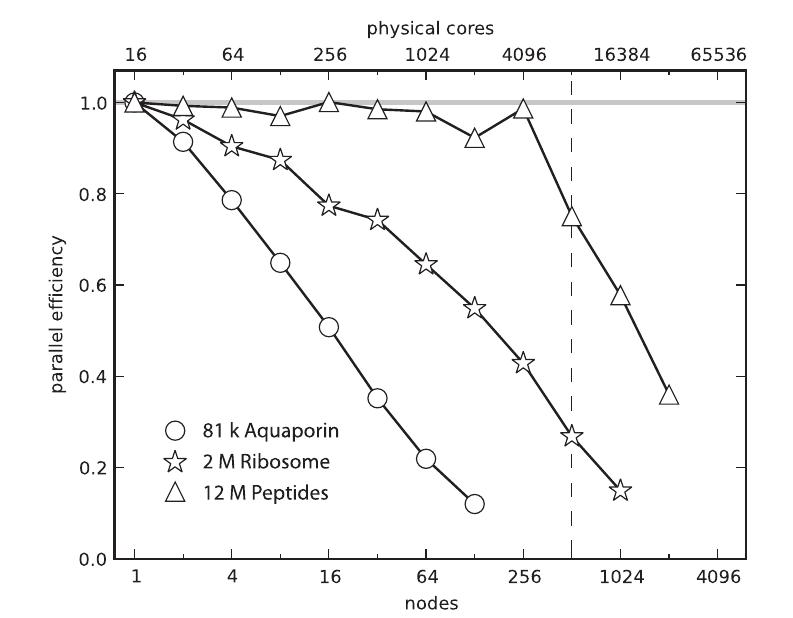
\includegraphics[scale=0.6]{scalingMUC}
 \centering 
\caption{ Parallel efficiency of three GROMACS MD simulations of different size (81k - 12M particles). The parallel efficiency on N nodes is the execution time $t_1$ divided by N times the execution time on N nodes. $E_N = t_1 / (N\cdot t_N)$. Horizontal grey line indicates perfect scaling.}
\label{fig:scaling}
\end{figure}



\section{Tree-based methods}

Now we will look at an algorithm that scales linearly with the number of charges $N$ and which does not have inherent parallel communication bottleneck as \cite{kutzner2013scaling}.
Furthermore, it can be applied to systems with periodic as well to systems with open boundaries. Since it approximates the actual charge distribution by a set of multipoles, it is called the "Fast Multipole method" (FMM). It is also interesting to say that the FMM method has an error bound estimator which allows the error of the FMM to be controlled as shown \cite{dachsel2010corrected}
    
	\subsection{Mathematical preliminaries}
	
	Let's move back to the potential created by a charged particle :
	
	\begin{equation*}
	V = \frac{1}{d}
	\end{equation*}
	
	Let two particles $A(a,\alpha,\beta)$ and $R(r,\theta,\phi)$, separated by a distance $d$: The distance between the particles is $d = |a - r|$.
	We would like to achieve is to "factorize the addition", having a product of one function depending only on $a$ and one depending only on $r$.
	
	
\begin{figure}[H]
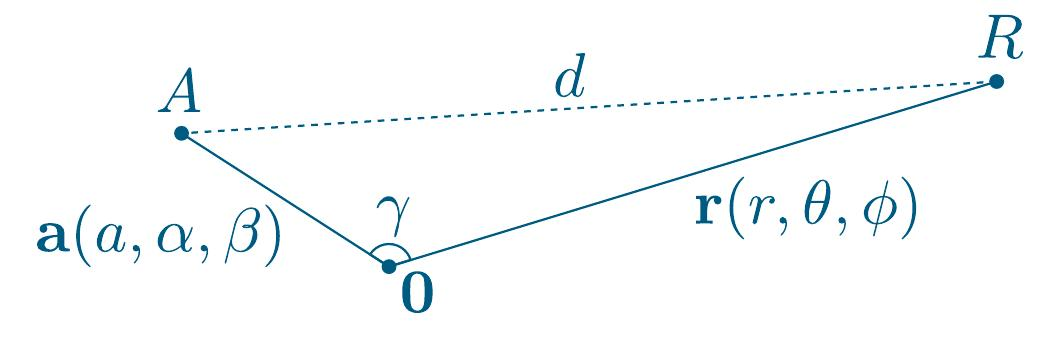
\includegraphics[scale=0.4]{distance}
 \centering 
\caption{Two particles $A(a,\alpha,\beta)$ and $R(r,\theta,\phi)$, separated by a distance $d$}
\label{fig:poster}
\end{figure}	
	
	
	The inverse distance can be written as :
	
	\begin{equation*}
		\frac{1}{d} = \frac{1}{|a-r|} = \frac{1}{\sqrt{a^2 + r^2 - 2ar \cos(\gamma)}}
	\end{equation*}

	This distance can then written as a series of Legendre polynomials  $P_l(u)$ of degree $l$ if $r \gg a$ :
	
	\begin{equation}
		\frac{1}{d} = \frac{1}{\sqrt{a^2 + r^2 - 2ar \cos(\gamma)}} = \sum\limits_{l=0}^{+\infty} P_l(u)\mu^l
	\end{equation}
	
	
	where $\mu = \frac{a}{r}$ and $u = \cos{\gamma}$ .
	
	with some manipulation as explained \cite{phdIvo} , we obtain : 
	
	\begin{equation}
	\frac{1}{|r - a|} = \sum\limits_{l=0}^{+\infty} \sum\limits_{m = -l}^{+l} \frac{(l-m)!}{(l+m)!} \frac{a^l}{r^{l+1}} P_{lm}\cos{(\alpha)}P_{lm}\cos{(\theta)}e^{-im(\beta - \phi)}
	\end{equation}
	
	in order to approximate the scheme, we can truncate the infinite series to a certain order $p$, we call this order the \textbf{multipole order}
	
	\begin{equation}	
	\frac{1}{|r - a|} \simeq \sum\limits_{l=0}^{\textcolor{red}{p}} \sum\limits_{m = -l}^{+l} \frac{(l-m)!}{(l+m)!} \frac{a^l}{r^{l+1}} P_{lm}\cos{(\alpha)}P_{lm}\cos{(\theta)}e^{-im(\beta - \phi)}
	\label{eq:order}
	\end{equation}
	
	We can now rewrite the summation the following way :
	
		\begin{equation}
	\frac{1}{|r - a|} \simeq \sum\limits_{l=0}^{p} \sum\limits_{m = -l}^{+l}
	\underbrace{\frac{a^l}{(l+m)!} P_{lm}(\cos(\alpha))e^{-im\beta}} _{O_{lm}(\textbf{a})}
    \underbrace{\frac{(l-m)!}{r^{l+1}} P_{lm}(\cos(\theta))e^{+im\phi}} _{M_{lm}(\textbf{r})}
	\end{equation}
	%and ${M_{lm}(\textbf{r})$
	hence,
	
		\begin{equation}
	\frac{1}{|r - a|} \simeq \sum\limits_{l=0}^{p} \sum\limits_{m = -l}^{+l}
	{O_{lm}(\textbf{a})}
    {M_{lm}(\textbf{r})}
	\end{equation}
	
	
	Thus it is possible to "factorize" the inverse of the the distance $\frac{1}{d}$ so we can obtain two independent terms ${O_{lm}(\textbf{a})}$ and ${M_{lm}(\textbf{r})}$  for two particles 


	We can then define the multipole moment $\omega_{lm}(q,\textbf{a}) = q O_{lm}(\textbf{a})$ and the Taylor-like moment $\mu_{lm}(q,\textbf{r}) = q M_{lm}(\textbf{r})$
	
	One obtains the following "bipolar expansion" for two particles associated with two different origins :
	
    \begin{equation}
    \frac{1}{|\textbf{a}_1 - \textbf{a}_2 + \textbf{R}|} = 
    \sum\limits_{l=0}^{+\infty}
    \sum\limits_{j=0}^{+\infty}
    \sum\limits_{m=-l}^{+l}
    \sum\limits_{k=-j}^{+j}
    (-1)^j \cdot O_{lm}(\textbf{a}_1) \cdot M_{l+j,m+k}(\textbf{R}) \cdot O_{jk}(\textbf{a}_2)
    \end{equation}



	\begin{figure}[H]

    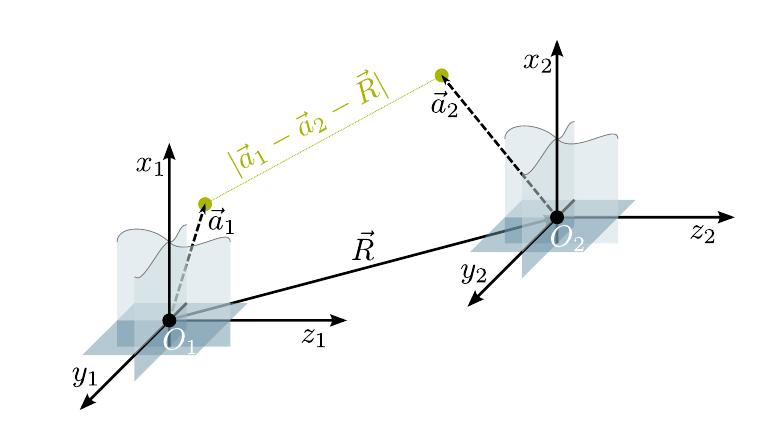
\includegraphics[scale=0.7]{bipolar}
    \centering 
    \caption{Scheme of two particles expanded according to two different origins}
    \label{fig:bipolar}
    \end{figure}




	
	\subsection{Workflow of the algorithm}
	
	Once some mathematical preliminaries are set, it is possible to explain the workflow of the algorithm.
	
	\subsubsection{Splitting the Space}
	
	One of the ideas of the FMM is to approximate far-away charges by multipoles expansions,whereas interactions between near charges are calculated directly without any approximation. So that's why we need to split the simulation box in sub-boxes, so that near field and far field contributions can be computed everywhere. 	
	
	So first step of the scheme is to split the space in order to generate different groups. The idea is to recursively split the space in eight octants, created the so-called structure of an \textit{octree}. So the number of boxes is $8^{D-1}$, where $D$ is the depth of the oct-tree.
	
		
	
	\begin{figure}[H]
	    
    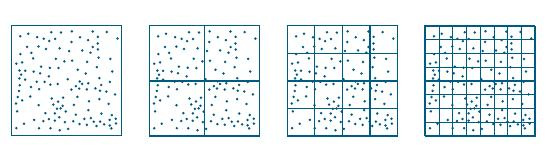
\includegraphics[scale=0.9]{BoxDepth}    
    \centering 
    \caption{Example of a division of the space in boxes. The  example is in 2D so the structure of the space is called a \textit{quadtree}.}
    \label{fig:depth}       
     \end{figure}
	
    
    The number of subdivisions is called the \textit{depth} $D$. For example, in figure \ref{fig:depth}, we can observe from left to right the depths $0,1,2$ and $3$.
    
    Then each particle is assigned  to the box of lowest depth it is found in.
    
	\subsubsection{Defining a Separation Criterion}
	
	For the further computations it is needed to define a separation criterion $ws$: It is the $ws^{th}$ next neighbors of a given depth. Two boxes A and B are called \textit{next neighbors} is they are at the same level and box B is enclosed by a box of size $(2 ws + 1)^3$ around the center of A 
	
	
	
	
	\begin{figure}[H]
    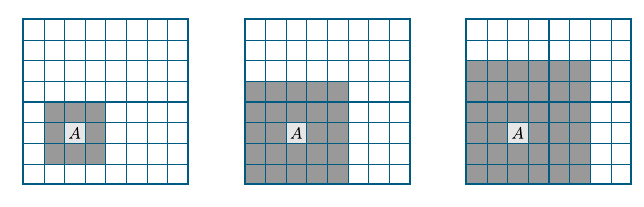
\includegraphics[scale=0.7]{separation}    
    \centering 
    \caption{Example of the influence of the separation criterion $ws$ for a given box $A$, from left to right, $ws = 1,2,3$. (from \cite{phdIvo})}    
    \label{fig:separation}
     \end{figure}
	
		This separation criterion divides the space into two parts. If two particles are close so they are in the same grey space as defined figure (\ref{fig:separation}), then, their interaction is computed directly, otherwise their interaction is approximated via multipoles.
	
	It is most of the time not possible to set the separation criterion $ws$ to 0, as the multipole expansion might overlap. Using a bigger $ws$ means that the order of the multipole expansions need to be less important for the same precision, however this will increase the number of direct $\mathcal{O}(N^2)$ operation, which are  more computationally expensive.       
    
    
	The algorithm by itself will be done in separate phases we call "passes" : there will be 4 different passes:
	
	\begin{description}
	\item[PASS 1] : Computing the Multipole moments
	\item[PASS 2] : Transforming distant expansions into multipoles
	\item[PASS 3] : Shift Taylor-Like expansions down the tree
	\item[PASS 4] : Computing forces and Energies
	
	\end{description}
		
	
	    
    
    
    \subsubsection{PASS 1 : Computing the Multipole moments}
    
    Once every particle is assigned to its box at the lowest level, we will compute the multipole moment $\omega_{lm}^j$ of each box.
    
    \begin{equation}
    \omega_{lm}^{j}(q,\textbf{a}) = q^j a_j^l \widetilde{P}_{lm}(\cos(\alpha_j))e^{-im\beta_j}
    \end{equation}
%
To construct the multipoles at the higher levels from the existing multipoles at the lowest level, each multipole order is moved to the Center of the parent box using the so-called $M2M$ (Multipole to Multipole) operator:    
    
    \begin{equation}
    \omega(\textbf{a} + \textbf{b}) = \sum\limits_{j=0}^{k} \sum\limits_{k=-j}^{j} \omega_{jk}(\textbf{a}) O_{l-j,m-k}(\textbf{b})
    \end{equation}

   $O_{l-j,m-k}(\textbf{b})$ is called the $M2M$ operator.
   
   \begin{figure}[H]
   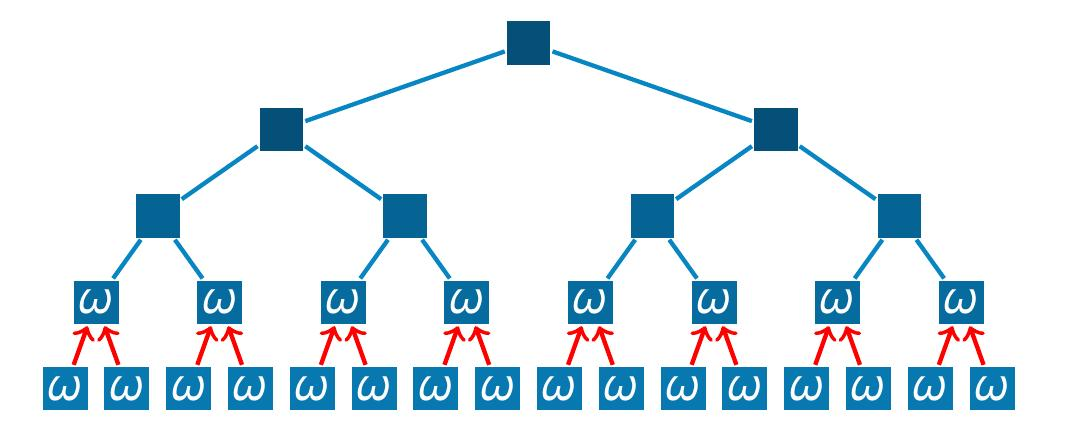
\includegraphics[scale=0.4]{ShiftMultipole}
    \centering 
    \caption{Example in 1-D showing the shifting of the multipole moments using the M2M operator. (from \cite{phdIvo}) }
    \label{fig:multipole}
   \end{figure}
   
   
   	\subsubsection{PASS 2 : Transforming distant expansions into multipoles}
   	
   PASS2 transforms distant expansions (beyond the separation criterion) $\omega_{lm}$ into a Taylor-like moment $\mu_{lm}$. This transformation is done over at most 189 boxes. This transformation is applied for each depth of the tree.  
   	
   	
 \begin{figure}[H]
 	\label{fig:M2L}
   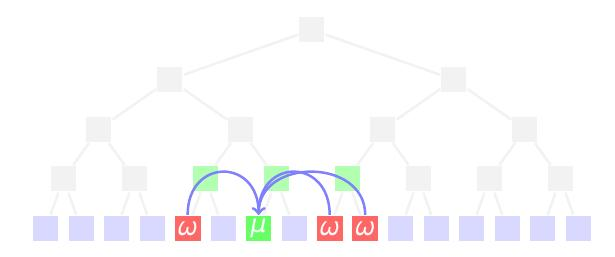
\includegraphics[scale=0.8]{transformExpansions1}
    \centering 
    \caption{Example in 1-D showing the transformation of distant expansions into multipoles (from \cite{phdIvo})}
    
   \end{figure}
   
	In order to compute this transformation, two different rules have to be applied:
	
	\begin{enumerate}	
	\item Take the non-separated parent boxes, as shown sub-figure (a) below.
	\item Then the children of the parent box are selected, taking into account the separation criterion for the child boxes.	
	\end{enumerate}	   
   
	 
 \begin{figure}[H]
   \subfloat[First, the parents of the box are chosen] {\label{fig:parentBox} 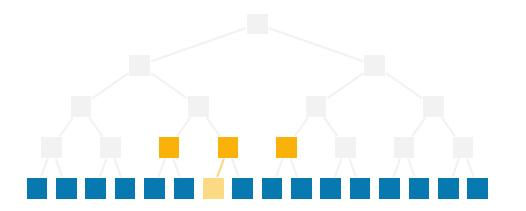
\includegraphics[scale=0.6]{transformExpansions2}}   
   \subfloat[Then, then children of the parents are chosen. Then the separation criterion can apply] {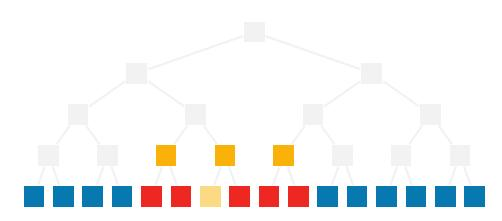
\includegraphics[scale=0.6]{transformExpansions3}}
    \centering 
    \caption{Interation Rules for the transformation of the multipole expansions (from \cite{phdIvo})}
    \label{fig:multipole}
   \end{figure}   
   
	  Mathematically, the transformation from multipole expansions to multipole moments is given using the  M2L (Multipole to Local) Operator
	  
	  \begin{equation}
	  \mu_{lm}(\textbf{b} - \textbf{a}) = \sum\limits_{j = 0}^{+\infty} \sum\limits_{k=-j}^{j}
	  M_{j+l,k+m}(\textbf{b}) \cdot \omega_{jk}(\textbf{(a)})
	  \end{equation}
   
   	where $M_{j+l,k+m}(\textbf{b})$ is the M2L operator : It allows to exchange, as figure (\ref{fig:M2L}) shows, information between boxes of the same level.

\subsubsection{PASS 3 : Shift Taylor-Like expansions down the tree}

Once the local $\mu_{lm}$ expansions are computed, the expansion are shifted to the lowest level of the tree using the L2L (Local to Local) operator.

	\begin{figure}[H]
	\label{fig:L2L}
   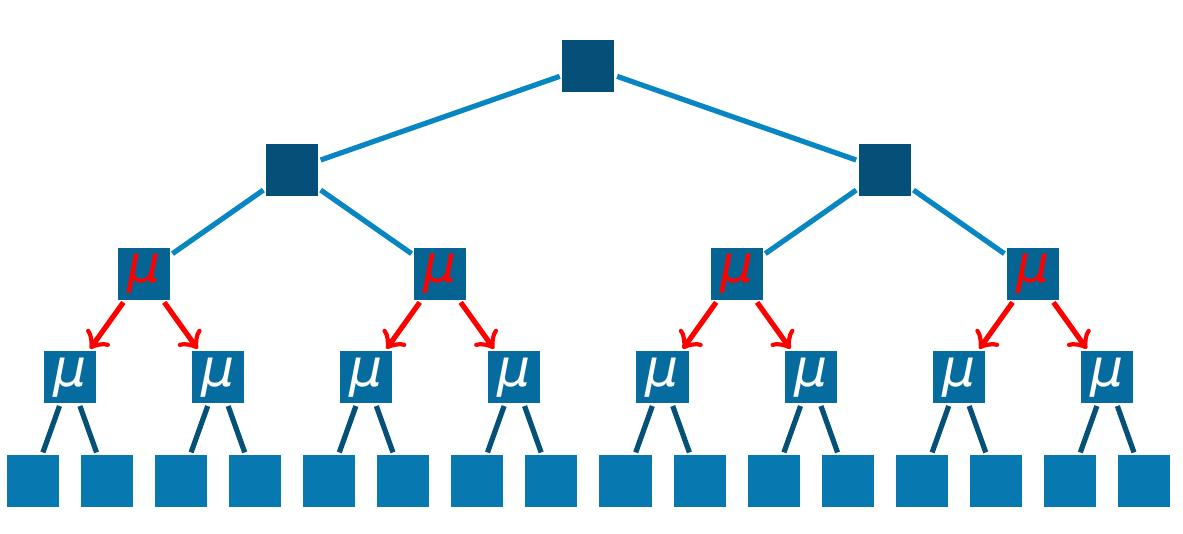
\includegraphics[scale=0.4]{L2L_1}
    \centering 
    \caption{Example in 1-D showing the shifting of the local moments using the L2L operator. (from \cite{phdIvo}) }
    
   \end{figure}
    
 	This shift operation is done by the following formula :
 	
 	  \begin{equation}
	  \mu_{lm}(\textbf{r} - \textbf{b}) = \sum\limits_{j = l}^{p} \sum\limits_{k=-j}^{j}
	  O_{j-l,k-m}(\textbf{b}) \cdot \mu_{jk}(\textbf{(a)})
	  \end{equation}
 
 		where $O_{j-l,k-m}(\textbf{b})$ is the L2L operator : It allows to exchange, as figure (\ref{fig:M2L}) shows, information between levels downwards.
 		
 \subsubsection{PASS 4 : Computing forces and Energies}
 
 
 After PASS 3, we have in every box at the lowest level both the multipole expansion as well as the local expansion, thus everything to compute the far-field contribution to the forces and the potential of the system. 
 
\begin{figure}[H]
	\label{fig:farfield}
   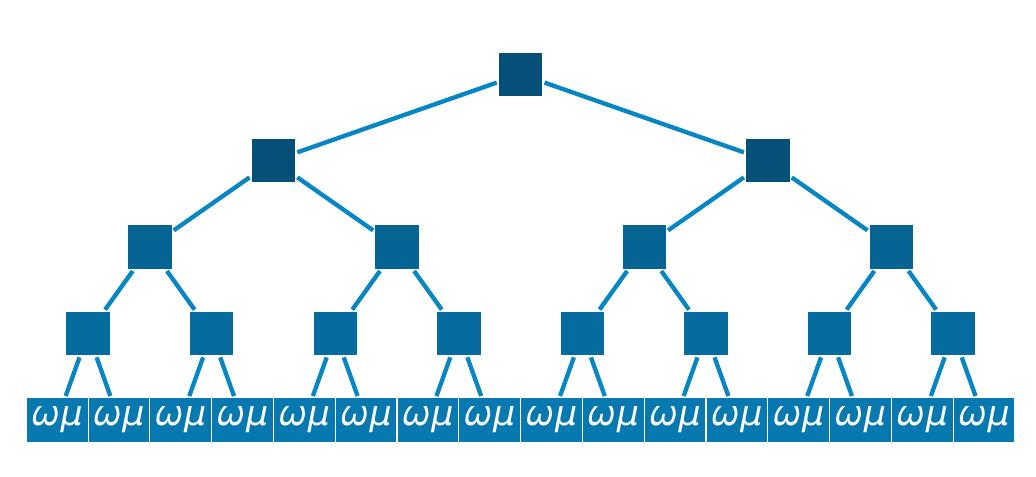
\includegraphics[scale=0.5]{farfield}
    \centering 
    \caption{Situation after PASS 3 }
    
   \end{figure} 
   

   
   So we have for the electric field :
      
   \begin{equation}
   E_{FF} = \sum\limits_{l=0}^{p} \sum\limits_{m=-l}^{+l} \mu_{lm}(\textbf{r}) \omega_{lm}(\textbf{a})
   \end{equation}
   
   For the potential :
 
 	\begin{equation}
   \Phi_{FF} = - \sum\limits_{l=0}^{p} \sum\limits_{m=-l}^{+l} \mu_{lm}(\textbf{r}) \nabla_{\textbf{a}_i}[a_i^l \widetilde{P}_{lm}(\cos\alpha_i)e^{-im\beta_i}]
   \end{equation}
   
   and for the force :
   
   \begin{equation}
   \textbf{F}_{FF} = - \sum\limits_{l=0}^{p} \sum\limits_{m=-l}^{+l} \mu_{lm}(\textbf{r}) \nabla_{\textbf{a}_i}[a_i^l \widetilde{P}_{lm}(\cos\alpha_i)e^{-im\beta_i}]
   \end{equation}
   
 Then the near-field contribution can be easily computed : 

 

\chapter{Comparing FMM and PME accuracy}

    In this chapter I will more precisely explain my work done in the Lab, which consisted in comparing the PME methods, which is for example used by GROMACS, and the FMM method, used by a solver made between the Jülich Forschungszentrum and the Max Planck Institute for Biophysical Chemistry in Göttingen.

  


\section{Presentation of GROMACS}

    GROMACS (GROningen MAchine for Chemical Simulations) is a simulation software used for Molecular dynamics. It was originally developed in the Biophysical Chemistry department of University of Groningen but it is now developed around the world. GROMACS is made to be as fast as possible using all possible techniques to improve its performance (MPI, GPU computing) 
    
   
	\subsection{Structure of a File}
	
	 The program is used  by modifying text files that giving information on the structure of the system that has to be simulated and the parameters of the simulation. The files are the following 
	 
	\begin{itemize}
	
	\item The *.pdb file are the \textit{Protein DataBank} file : In this file is denoted the position and the type of the particles of the system. It also gives the size of the simulation box

	\item The *.top files (namely \textit{topology} files) are the file where the properties of the atoms are defined. These properties are for example the charge, the Van-der-Waals parameters or the binding forces of the system. This configuration is often done with force field files such as AMBER or CHARMM
		 
	\item The *.mdp (MD parameter file) files are defining the physical and computational parameters of the simulation. It is defining the methods used for the simulation. In our case we are mostly interested in the electrostatics part of the computation ; it is then possible to select the method (PME or Cut-Off methods) and the parameters for the PME
	
	\end{itemize}
		
	\subsection{PME parameters}
	
	In this paragraph I will explain the parameters it is possible to play with:
	
	\begin{enumerate}
	

	\item[\textbf{CutOff}] The first parameter is the CutOff : It allows to set the Cut-Off radius for the Cut-Off method, but it also sets the difference between the direct part and the reciprocal part in the PME method
	
	\item[\textbf{Fourier Spacing}] The other important parameter is the fourier spacing. I remind that in the PME method a 3D FFT is done in order to compute the energies and the forces of the system. The FFT is so computed on a grid : The dimension of the grid is given by the \textit{Fourier Spacing} parameter.
	
	\item[\textbf{PME Order}] The PME order gives the order of the charge interpolation on the grid. For instance, PMEorder$= 4$ corresponds to a cubic interpolation. 		
	
	\end{enumerate}
	
	\subsection{Command to launch a GROMACS simulation }	
	
The workflow to laumch a GROMACS Simulation is the following : 



First generate a .tpr binary file containing all the information about the simulation. The file is processed using the \textit{grompp} (Gromacs Preprocessor). The command is :


{\centering\tt {grompp -f mdpfile.mdp \\
	 -p topFile.top \\
	 -c pdbFile.pdb \\
	 -o tprFile.tpr \\ 
 }}

\vspace{5mm}
where the input files are the *.mdp , *.top and *.pdb (Respectively properties of the Simulation, of the atom, and the position of the Atoms). The *.tpr file is the output file.

It is then possible to run the simulation using the program mdrun, which as its name stands, runs the md simulation. A possible example is :

{\centering\tt { mdrun -s tprfile.tpr \\
				 -ntomp    4  			\\		
				 -ntmpi    4				 \\
				 -nsteps 0     		  \\  
 }}
 
\vspace{5mm}

Where the .tpr File is now the input file, containing everything about the simulation, -nsteps is the number of time steps needed (In the case of this Intership, no time intergration is needed as just the forces are required). It is also possible to choose the number of CPU cores needed for the simulation (Using MPI and OpenMP).

\section{Presentation of fmsolvr}	

	The software used to compute the electrostatic forces with the FMM is not GROMACS (at least not for the moment). It is developed by both the Max-Planck Institut for Biophysical Chemistry and the Jülich Forschungszentrum . In the following chapters, we will call this code \textit{fmsolvr}. 
	
	The codebase is mostly written in C++.  There exists several git branches for the program, allowing different versions of the system.	
The First version is a sequential version, which is the "basic" version of the FMM code . There also exists a version which allows periodic boundary conditions : We will use this version a lot as we need to compare it to the PME, which, by construction, uses periodic boundary conditions.	

The input file, is a *.hpp file containing 4 arrays of size $N$, where $N$ is the number of atoms in the simulation : one charge array $q$ , and three array $x,y,z$ for the positions of the atoms.

\subsection{FMM Parameters}

The simulation can be launched using the following command : 

\begin{verbatim}
DEPTH=${DEPTH}  MULTIPOLEORDER=${MULTIPOLEORDER}  WS=${WS} 
OPENBOUNDARY=0 UNITBOX=${UNITBOX} CENTER=c 
./fmmtest $inputFile.qxyz $outputFile.dat \\	

\end{verbatim}

{\centering\tt { DEPTH=\${DEPTH}  MULTIPOLEORDER=\${MULTIPOLEORDER}  WS=\${WS} \\ 
OPENBOUNDARY=0 UNITBOX=\${UNITBOX} CENTER=c \\
./fmmtest \$inputFile.qxyz \$outputFile.dat \\					
 }}

The environment variables are the following :

\begin{description}
\item[DEPTH] The maximal subdivision of the space : if DEPTH=n the space will be divided in $8^{n}$ boxes.

\item[MULTIPOLEORDER] The Order of truncation in a the series as shown \ref{eq:order}
	
	where the multipole order is the red \textcolor{red}{p} in the first summation.
	
	
\item[WS] This gives the separation criterion $ws \geq 1$, which separates the far-field computation from the near space.

\item[OPENBOUDARY] if OPENBOUNDARY = 0, periodic boundary conditions will be used, if OPENBOUNDARY=1, then openbondaries will be used.

\item[UNITBOX] Gives the size of the simulation box (in nm).

\end{description}
 	
\section{Comparing GROMACS(PME) and fmsolvr(FMM) }	

The first part, if we want to make the PME and the FMM comparable, is to use the same simulation for both programs, hence requiring coding some tools transforming a GROMACS-compatible file to fmsolvr-compatible one. Then, we saw that the results we obtained weren't good enough as one system was using some dipole correction, so we needed to implements the dipole correction to the FMM system.

\subsection{File manipulation}

In this section will be explained the file modifications needed in order to have the simulations comparable on both systems.

\subsubsection{Making GROMACS only compute electrostatics forces}

In this Internship we just want to compute the electrostatic forces on our system. However, what we obtain in the GROMACS output file is the sum of all forces on each atom. These forces may include forces such as for instance Lennard-Jones potentials.
($V_{LJ} = 4\epsilon [(\frac{\sigma}{r})^12 - (\frac{\sigma}{r})^6] $). 

So the first thing to do is to modify the topology file (*.top), so there is no more Lennard Jones potential at all ; this snippet is added to the *.top file:


\begin{verbatim}
[ atomtypes ]
type atnum         mass   charge ptype           sigma  epsilon\\
  CLA    17    35.450000    0.000  A  0.000000000000  0.00000\\
  SOD    11    22.989770    0.000  A  0.000000000000  0.00000\\

\end{verbatim}


In the expression of the potential, we set $\epsilon = 0$ and $\sigma = 0$, so it gives $V_{LJ} = 0$. So we have modified the files such that there is only the electrostatic interaction at play in the simulation.

\subsubsection{Assure compatibility between *.qxyz and *.pdb files}

The next thing to do is to have the same simluation system for both methods : So I needed to make a few scripts to transform a *.pdb file in a *.qxyz or a *.hpp file.

The scripts are written in python, the workflow is the following:

{
	\centering 
	{
	
	  *.hpp $\xleftarrow{\tt{qxyz2hpp.py}}$  *qxyz $\xrightarrow{\tt{qxyz2gromacs.py}}$ *.pdb	
	}
}

So it is now possible to move the positions of the atoms one software to another software. (PME to FMM or FMM to PME)

\subsubsection{Output positions and forces to a Text file for GROMACS}

The last preliminary thing to do is to make the GROMACS Simulation print the positions and the forces in an easy and detailed way. We decided to modify the Gromacs code after the so-called {\tt{do\_force(...)}} function, which computes the forces for the system, a routine that prints the force as well as the positions in order to be
 easily used afterwards. 

\section{Dipole Correction}

\subsection{Silicamelt computation}

The first thing we did afterwards it to take a good precision for both methods and compare the forces.


The model we are using is called the "Silicamelt" system which is a system composed of $SiO_2$ atoms : It is a system comprised of about 100000 atoms. The silicon atoms (Si) have a $+2.4e$ charge and the Oxygen has a charge of $-1.2e$, where $e$ is the elementary charge $e \approx 1.6\cdot10^{-19} \text{C}$.
The size of the simulation box is $124.120$ nm in each dimension.

The parameters for the PME simulation are cutoff=1.2nm, PME order=12 and fourier spacing=0.015 nm. These parameters are the best obtainable for my workstation and are good enough to give a good approximation of the solution.

The paramerters for the FMM are : Depth=4, Multipole Order=40, and WS(Separation Criterion) =4. The simulations is done with periodic boundaries 

The relative error is computed the following way:

\begin{equation}
	error_{\text{relative}} = \frac{||F_{FMM} - F_{PME||}}{||F_{PME||}}
\end{equation}

The histograms are shown figure 4.3 and 4.4


	Some statistical information about the distribution gives us a maximum error of around 56\%, this maximum error is much bigger than the few percents expected and is therefore not acceptable.\\
	
	As shown figure (\ref{fig:magnitude}) we see the distribution of errors relative to the magnitude of the forces. Not unexpectedly, the biggest errors are recorded for smaller forces.

\subsection{Study of a two-particle system and dipole correction}
	In order to understand these big errors, we first decided to study how two particles behave. Then if the errors are small enough, it is possible to move to bigger systems.
	
We also observed that if we set 4 particles in a square in a quadrupole, so there is no dipole here, the value of the FMM system and the PME system are matching




 	
	
The hypothesis is that the dipole moment may be corrected in one system and not in another system. So the idea is to take two particles, one positively charged and the other negatively charged ; the two particles will form a dipole, with dipole moment $\vec{p}$ : 

\begin{equation}
	\vec{p} = q \vec{d}
\end{equation}	
	
	where $\vec{d}$ is the displacement vector pointing from the negative charge to the positive charge. 
	
	Then we can vary the distance between the two particles, compute the force using both the FMM method and the PME method and compare the force.	
	\begin{figure}
	   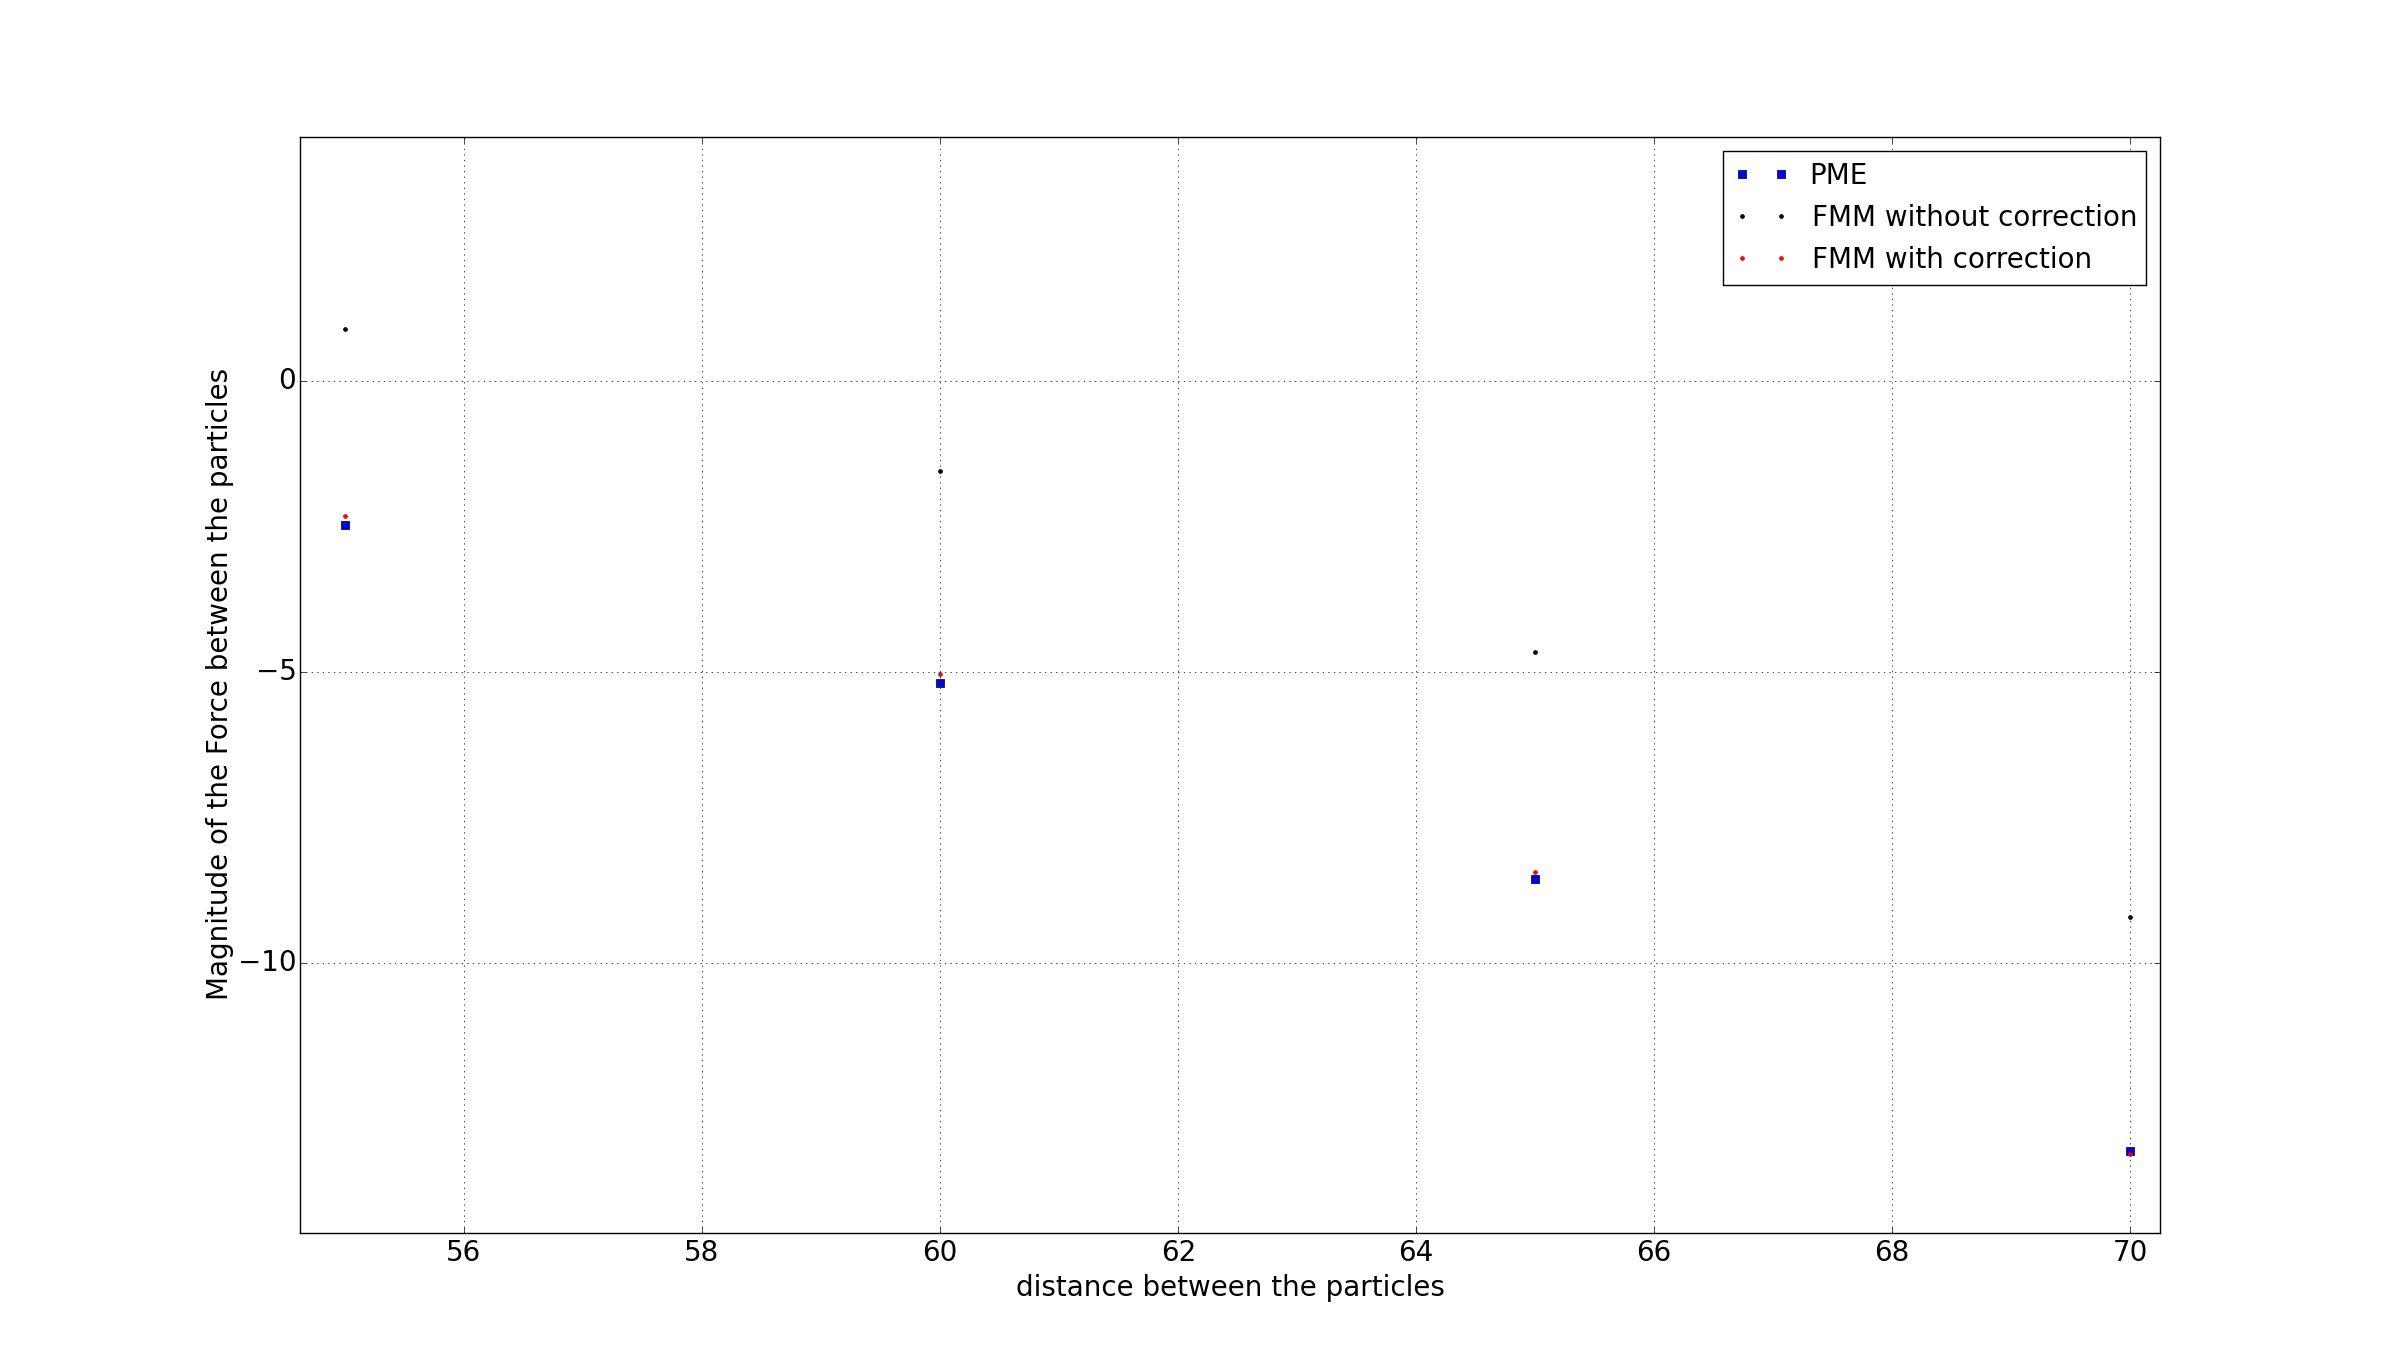
\includegraphics[scale=0.2]{dipoleCorrection}
    \centering 
    \caption{Figure representing the distance between two particles the x-axis (here 55,60,65,70 nm) and the  euclidean norm of the force for PME (Blue Square), FMM without correction (black) and with correction(red).
     It is possible to see that the dipole correction makes the FMM magnitude much closer to the PME.}    
   \end{figure}	
The dipole correction is done the following way :

It is possible to modify the potential in the FMM code using the following equation:

\begin{equation}
\label{eq:dipoleCorrection}
\nabla_iE_{\text{after correction}} = \nabla_iE_{\text{before correction}} - \frac{4\pi}{3 \cdot V} q_i \textbf{d}
\end{equation}	
	
	where V is the volume of the simulation box, $q_i$ the charge of the particle and $\textbf{d}$ is the dipole moment.

The dipole moment can be computed from the multipole moments, which contains the dipole moment : The multipole moments are contained in a triangluar array (because of symmetry and memory space reasons) the following way :

	\begin{figure}[H]
	\label{fig:triArray} 
	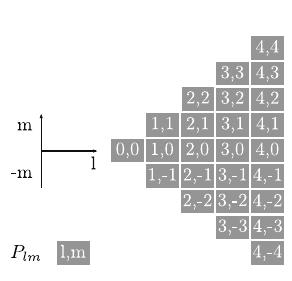
\includegraphics[scale=1]{triArray}
    \centering 
    \caption{Structure of the array containing the multipoles $\omega_{lm}\textbf{a})$ : the 'm' values are on the y-axis and the 'l'-values are on the x-axis. The dipole moment is contained in the boxes (1,1), (1,0) and (1,-1) }
   \label{fig:triArray}     
   \end{figure} 

As showed in figure (\ref{fig:triArray}), it is possible to obtain the dipole moment from the multipole ones, using the following formula :


%\vec{d}_x = -2 * \Re(\omega_{1,1})\\
%\vec{d}_y =  2 * \Im(\omega_{1,1})\\
%\vec{d}_z = -\Re(\omega_{1,0})

where $\Re()$ is the real part of the number and $\Im()$ is the imaginary part.

\begin{equation}
\hspace{10 mm}
\left\lbrace
\begin{array}{ccc}
\vec{d}_x = & -2 * \Re(\omega_{1,1})\\
\vec{d}_y = &  2 * \Im(\omega_{1,1})\\
\vec{d}_z = & -\Re(\omega_{1,0})
\end{array}\right.
\end{equation}

Then the correction can be applied using equation (\ref{eq:dipoleCorrection})\\


The C++11 code used for this correction, is the following :
	
	\begin{lstlisting}

for (size_t i = 0; i < n; ++i) {

	 auto cell_volume = (abc.a).x * (abc.b).y * (abc.c). z; // Only works with square Cell Unit
	std::cout << "Periodic Vector = " <<  (abc.a).x << std::endl;
	std::cout << "Volume " <<  cell_volume << std::endl;


	 std::cout << Real3(ordered_particles[i]) << "\t" <<reference_center << std::endl;

	 auto dr = Real3(ordered_particles[i]) - reference_center;
	 std::cout << "dr = " << dr << std::endl;

	 const auto& omega = tree_omega[0][0];
     dipole_moment.x =  -omega.get(1,1).real()*2;
	 dipole_moment.y = omega.get(1,1).imag()*2;
	 dipole_moment.z =  -omega.get(1,0).real();

	 // Potential Correction
	auto correction = (4.0*PI/(3.0 * cell_volume )) *  (dr.x * dipole_moment.x) + (dr.y * dipole_moment.y) + (dr.z * dipole_moment.z);
	std::cout << "Potential Before = " << potential[i] << std::endl;
	std::cout << "Correction = " << correction << std::endl;
	 potential[i] -= correction;
	std::cout << "Potential After = " << potential[i] << std::endl;
	 /*
	 efield[i].x -= 4*PI/3 * dipole_moment.x;
	 efield[i].y -= 4*PI/3 * dipole_moment.y;
	 efield[i].z -= 4*PI/3 * dipole_moment.z;
	 */



            Real q = -(-ordered_particles[i].s);  // negative gradient
            force[i] = efield[i] * q -  dipole_moment  * (4.*PI/(3.0*cell_volume)) * q  ;
	    Ec2 += q * potential[i];
        }
        Ec += Ec2 * 0.5;


\end{lstlisting}
	
\subsubsection{Back to the silicamelt simulation with dipole correction}

Now we can relaunch the simulation with the same parameters as before, including the dipole correction.
We obtain now a maximum error of 3.52\%, which is a much bigger improvement compared to the 56.35\% of the former simulation.

\begin{figure}[H]
  \label{fig:histogram}
    \centering  
 \subfloat[Histogram without correction] { \centering   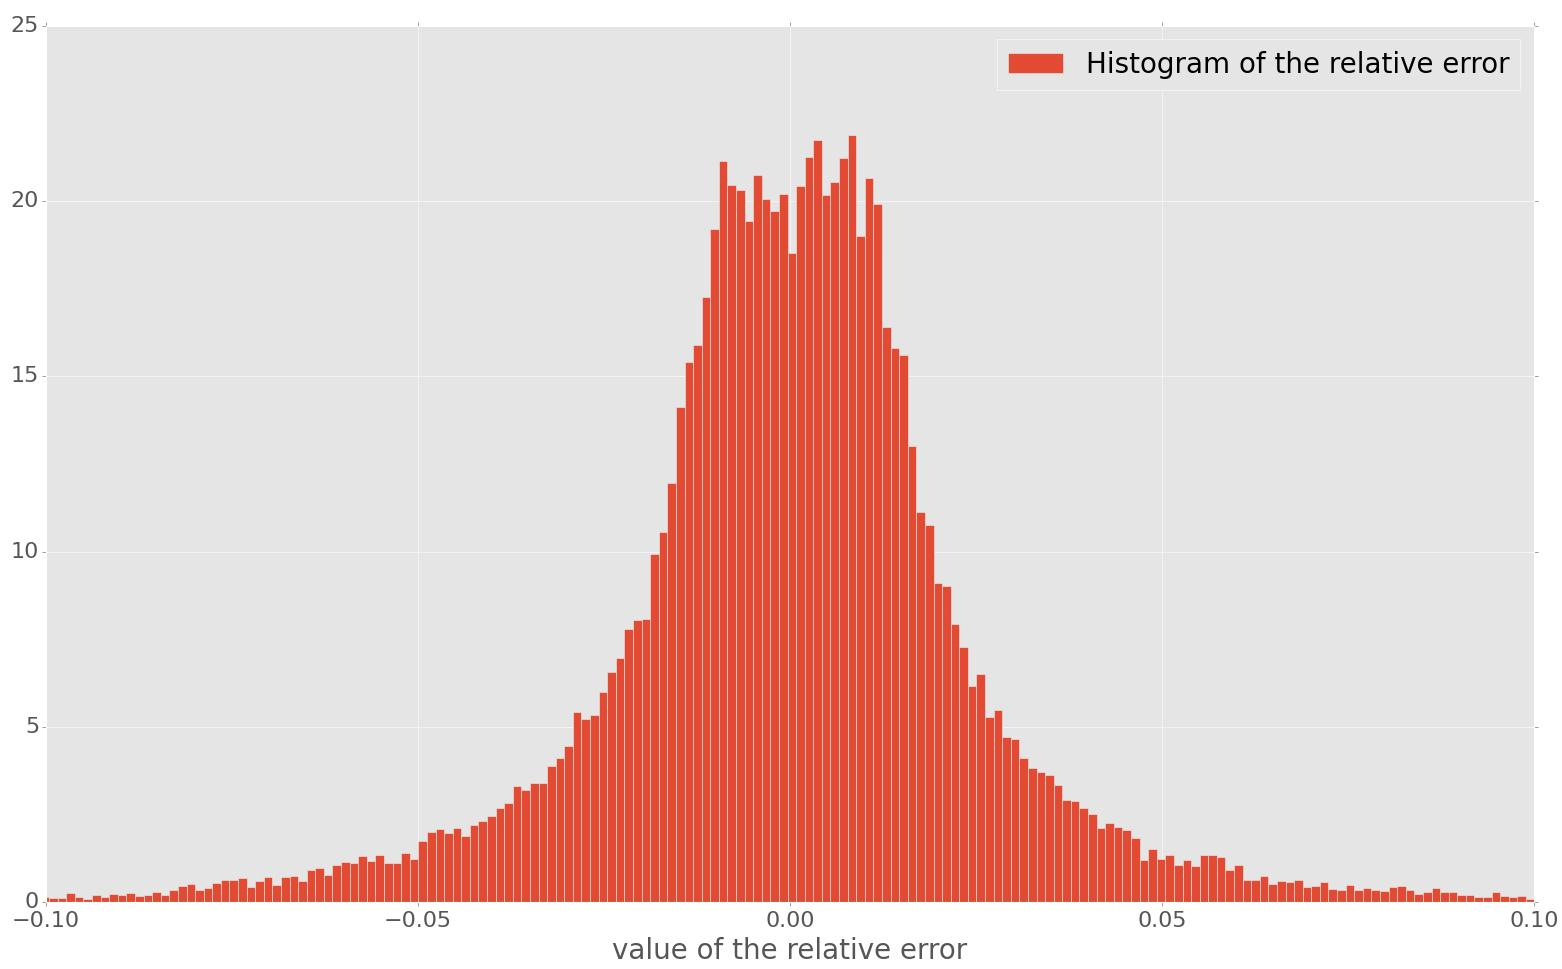
\includegraphics[scale=0.235]{hist_nocorrection}}\\    
  \subfloat[Histogram with correction] { \centering  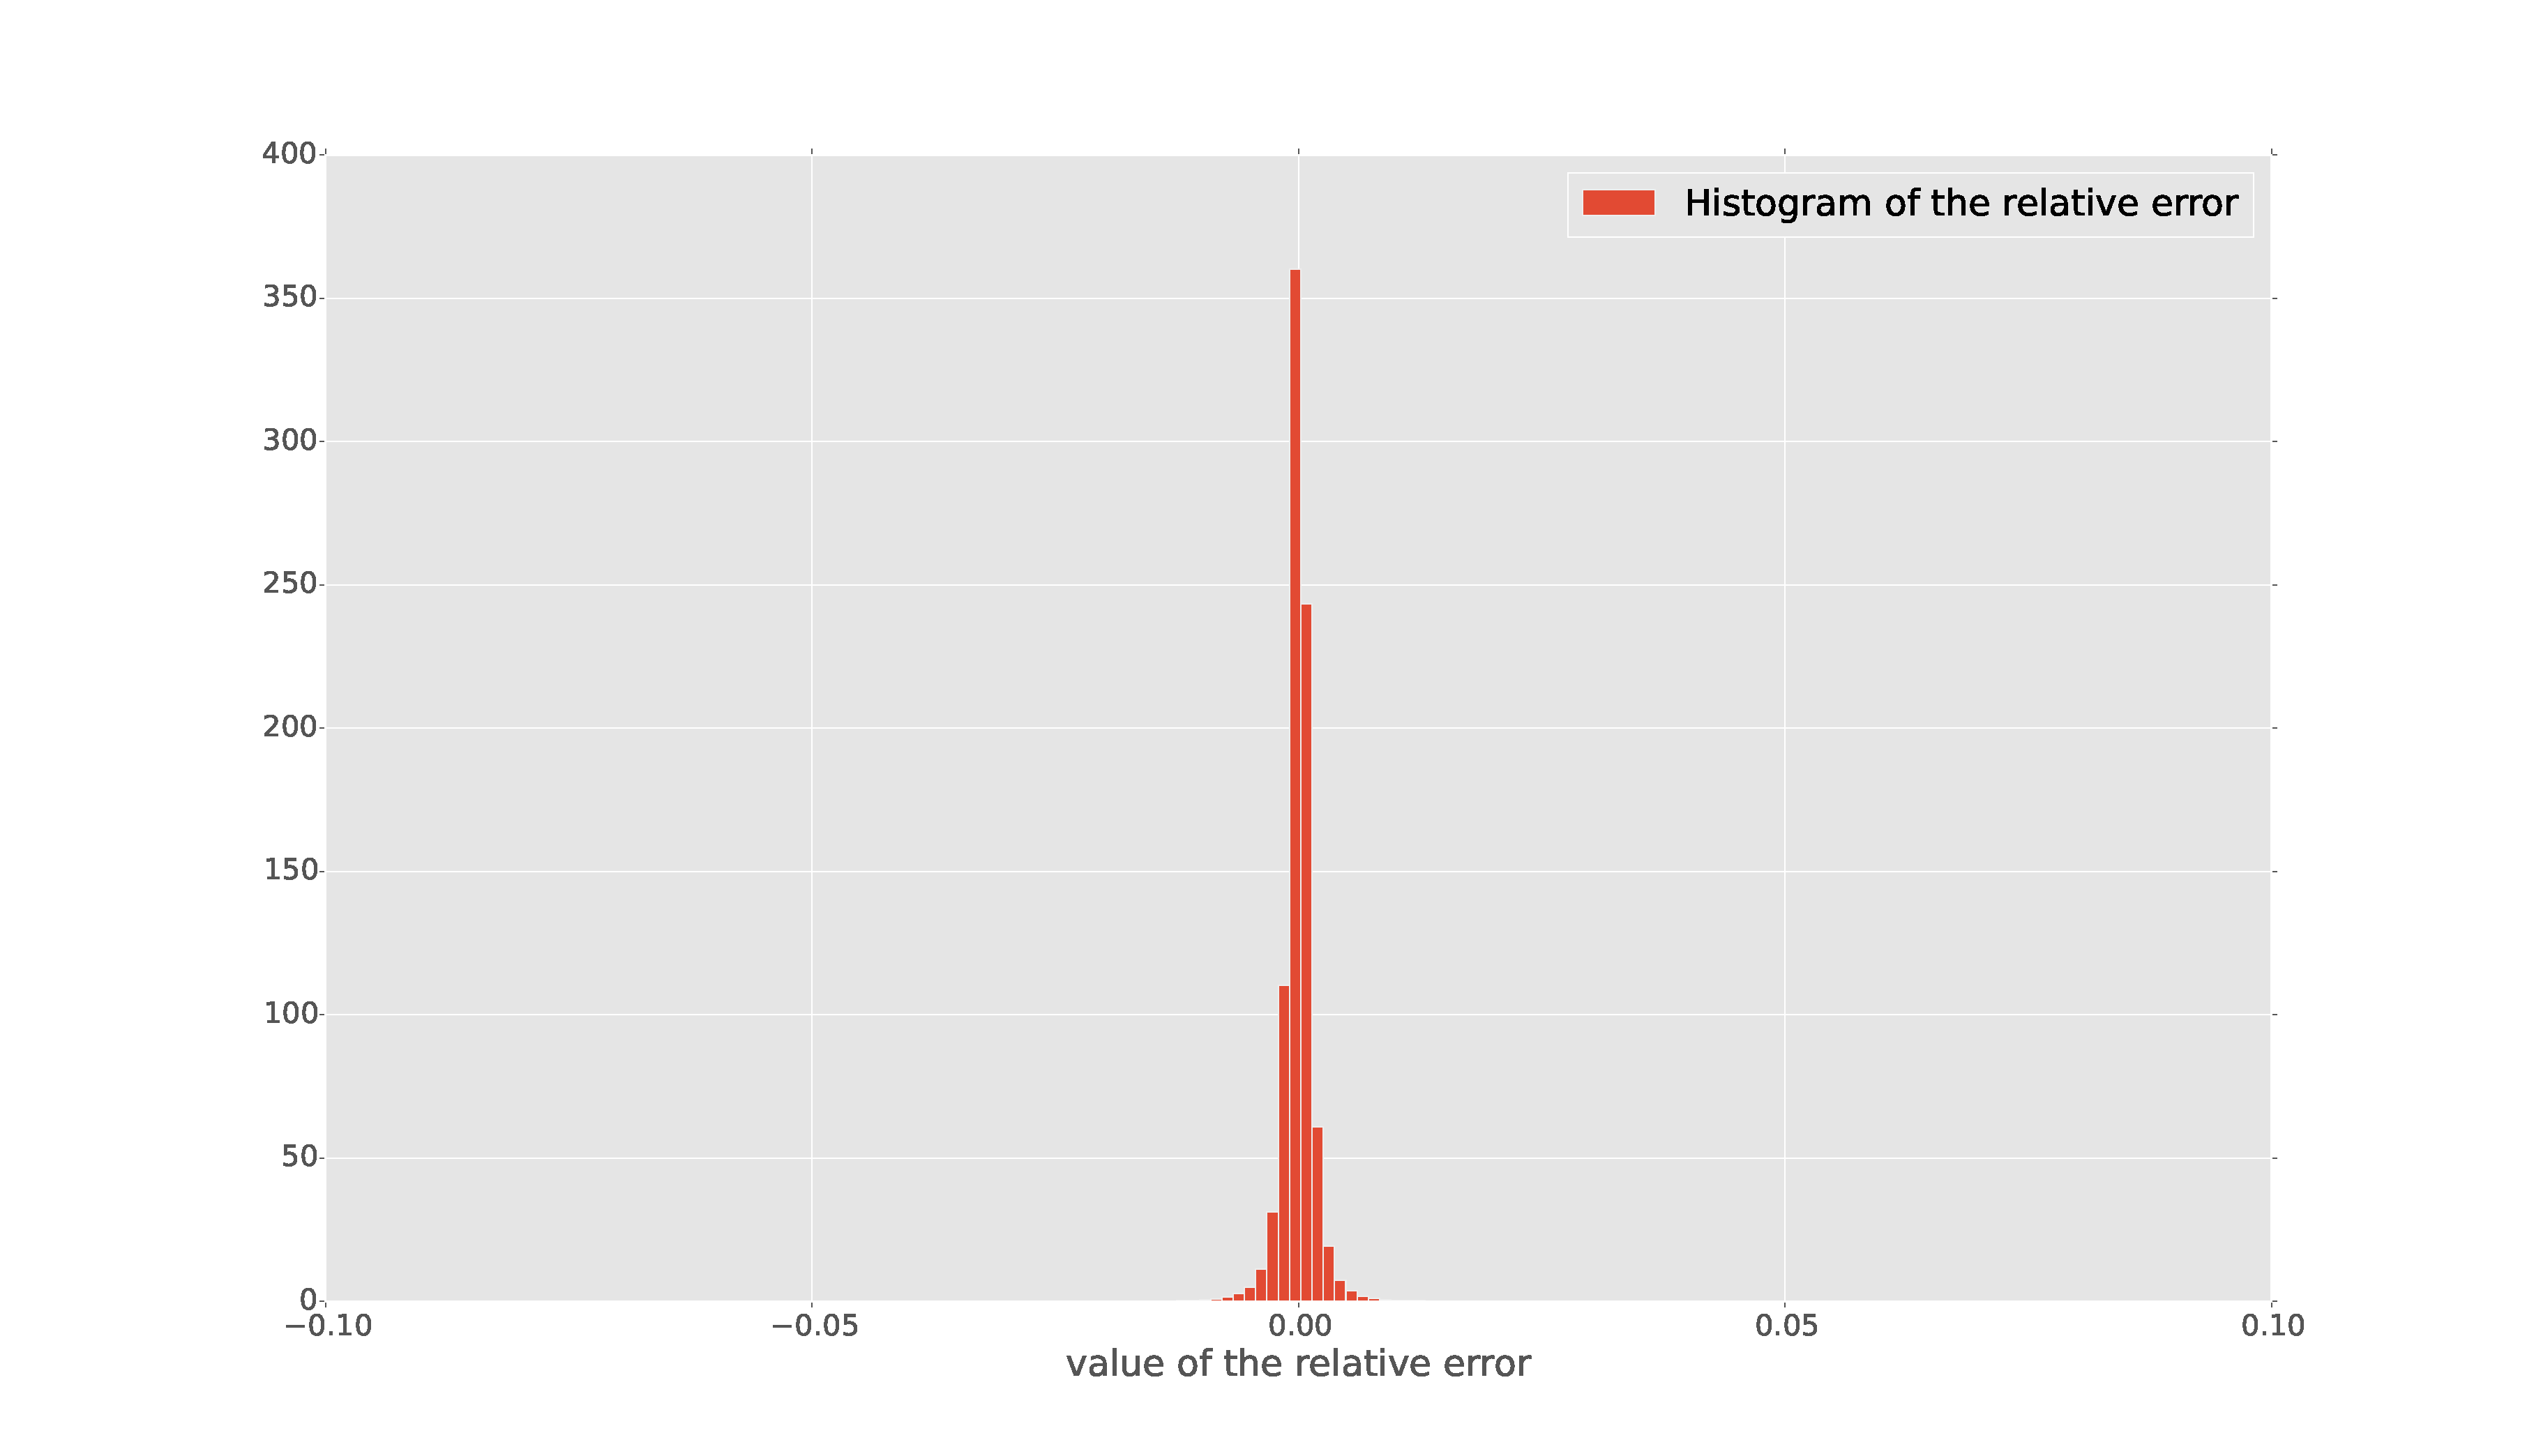
\includegraphics[scale=0.20]{hist_correction}}    
  
    \caption{Histogram representing the relative error for a silicamelt simulation : Top (a) histogram without dipole correction, bottom (b) with dipole correction.}    
   \end{figure}   







\begin{figure}[H]
	   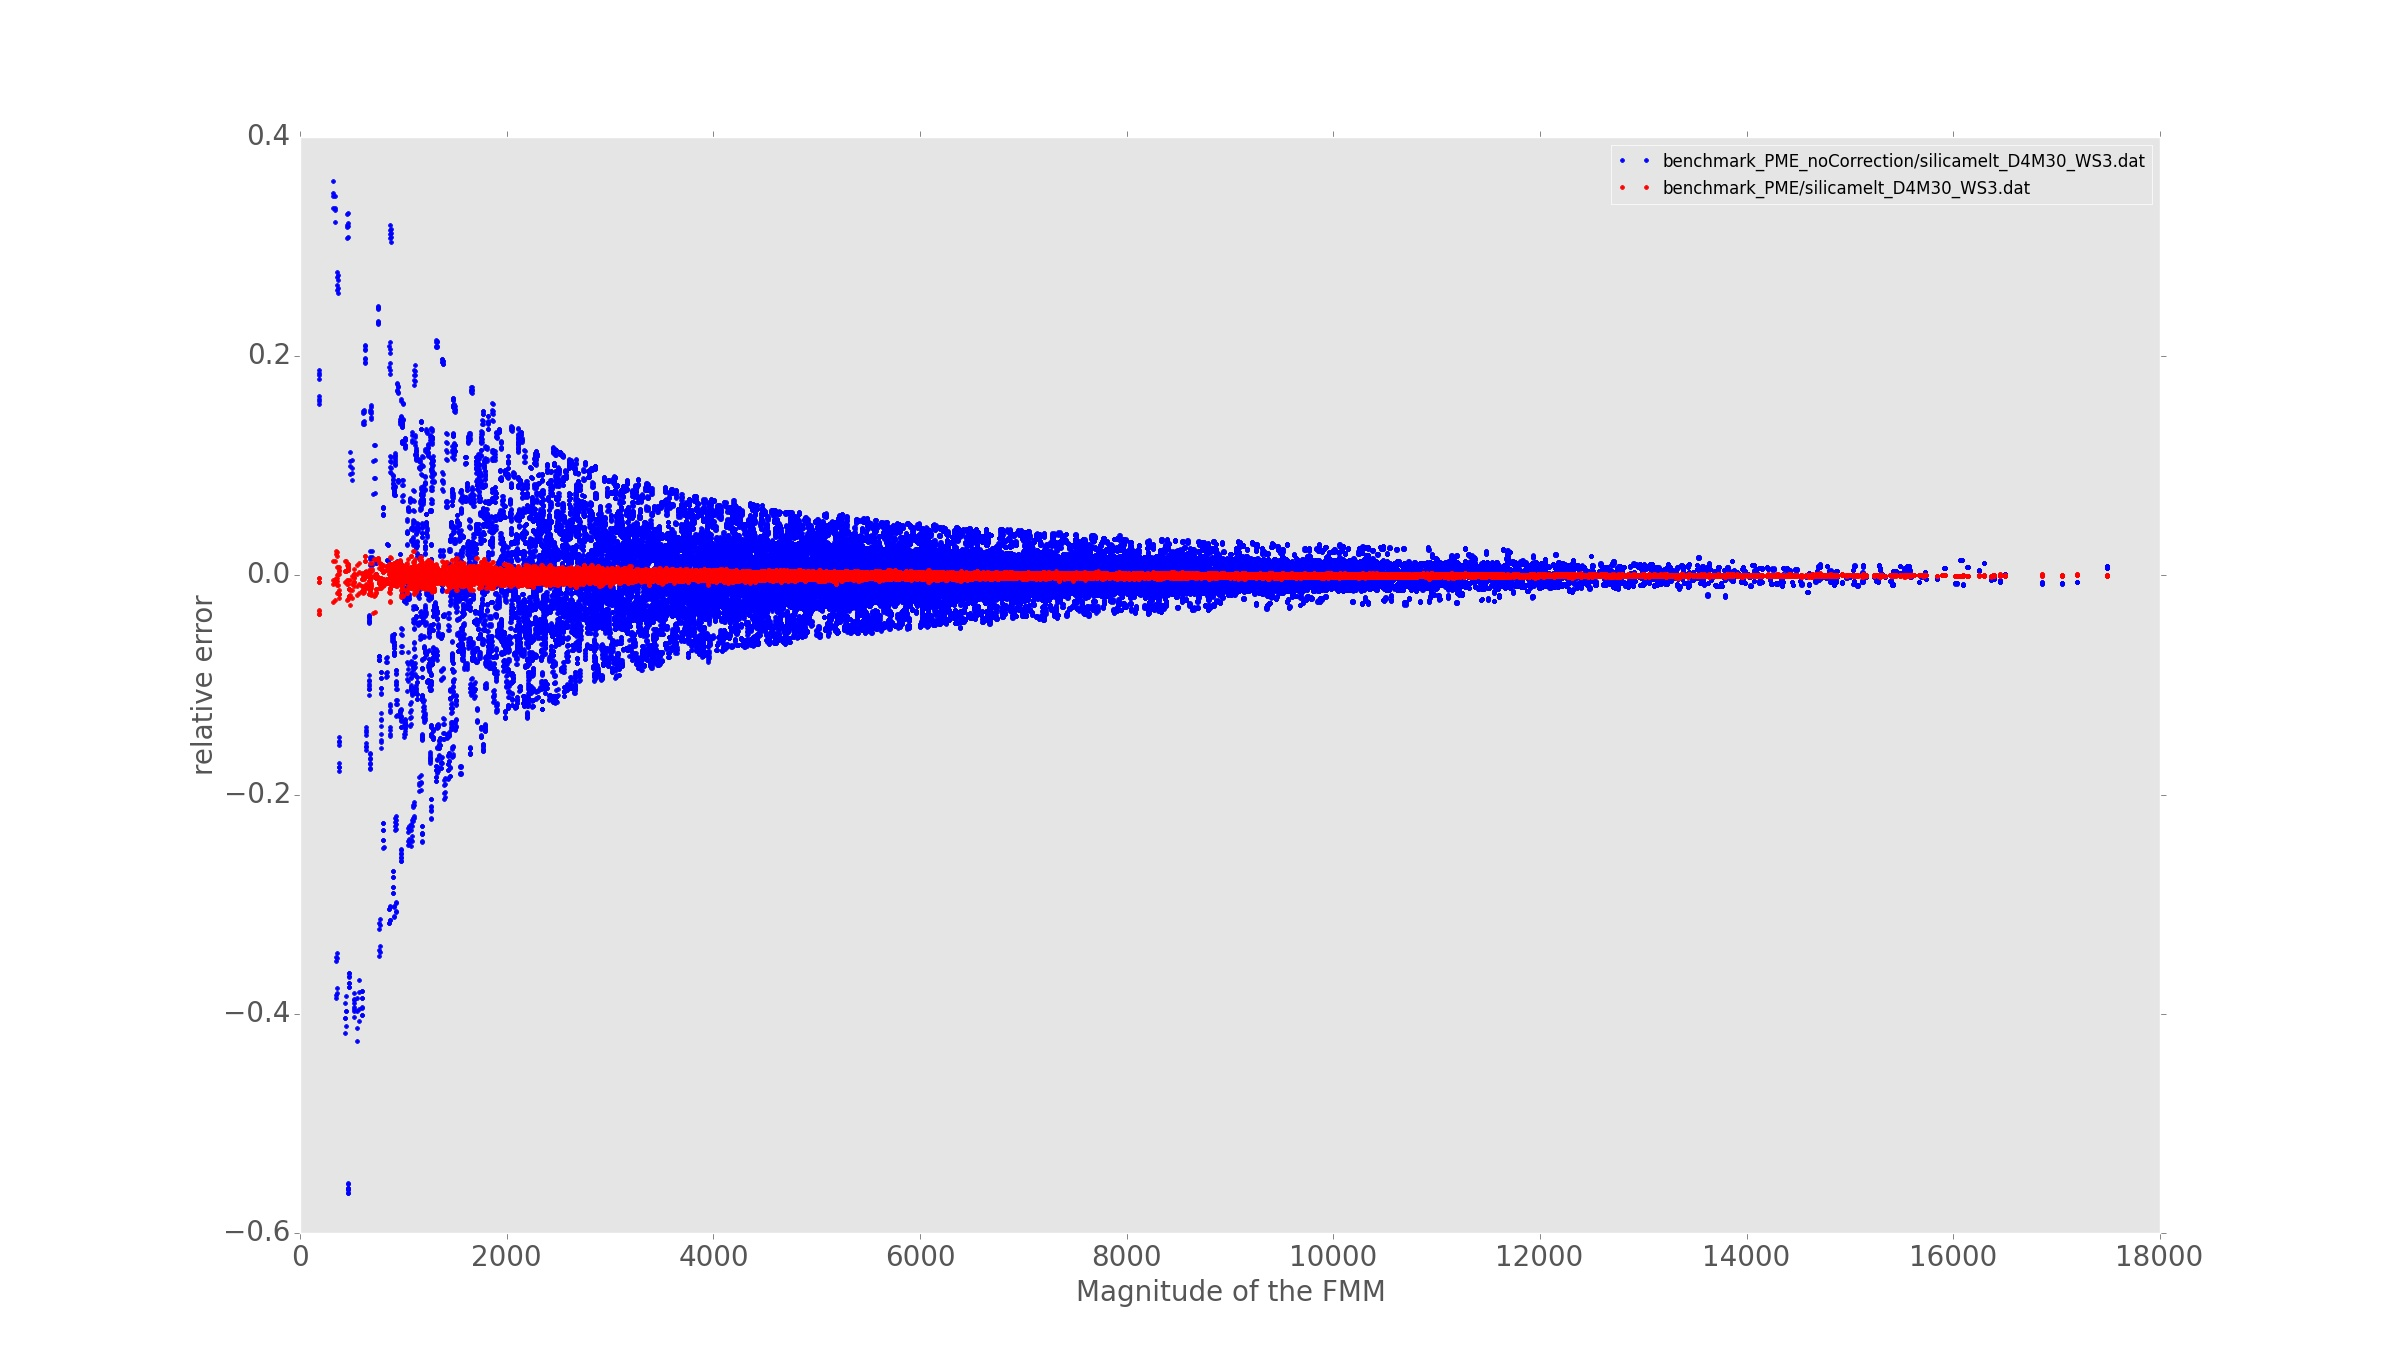
\includegraphics[scale=0.2]{magErr_Correction}
	    \label{fig:magnitude}
    \centering 
    \caption{Figure representing the Magnitude of the force on the x-axis and the relative error in the y-axis. The blue points represent the force before the dipole correction,then red points after the dipole correction.}    
    
    \label{fig:magnitude}
   \end{figure}  
   
\section{Comparing with an analytical solution : the NaCl system}

One other thing we want to try is to see the convergence of the scheme. The idea is to find out which set of parameters for the FMM has the same accuracy as a given set of parameters for the PME method. 

In order to study that, we want to have a system which is analytically solvable with periodic boundary conditions : That is why we decided to use a crystal as a system. 

\subsection{Generating the system}

The system used is based on a NaCl cristal structure. As a crystal is a stable structure, the total force acting on each atom has to be equal to 0. The potential felt by one atom can also be computed with a series ; this series converges to a value called the \textbf{Madelung Constant} which is equal for this crystal structure to approximately 3.495.

The generation is done with a python script writing the charges and the positions of the atoms in a *.qxyz file, then translated into a pdb file to obtain cristal structure necessary for GROMACS.

\begin{figure}[H]
	   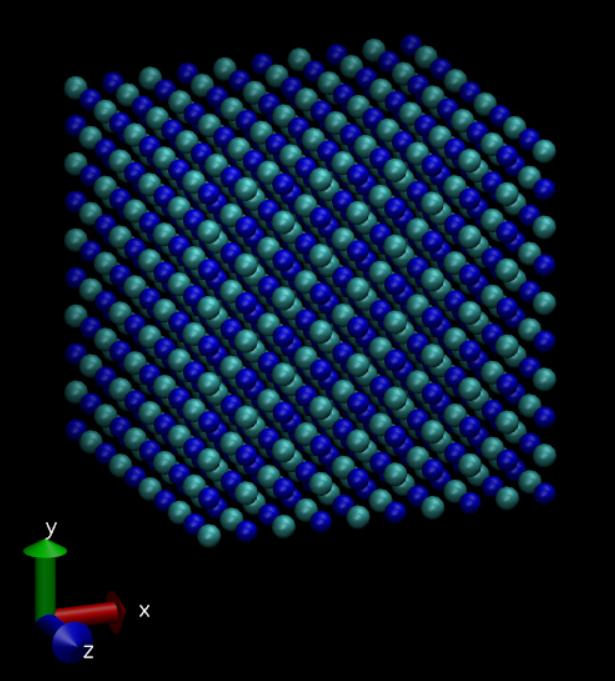
\includegraphics[scale=0.4]{nacl}
	   \label{fig:nacl_system}
    \centering 
    \caption{NaCl system generated with the script described above : The Blue atoms are Na atoms and the Green ones are Cl atoms. The Following image has been rendered using the visualization software VMD (Visual Molecular Dynamics)}    
   \end{figure}  


\subsection{Some explanations on the Owl cluster}

Now I will quickly explain how to submit a certain program to the cluster of the lab, which is called \textit{owl}.

Owl is the cluster of the lab used for the MD simulations : It contains about 12500 processor cores and 70 GPUs. The submit system is done using SGE (Sun Grid Engine).  

The cluster is accessible via an ssh connection : then it is possible to submit to the cluster using the following script:


\begin{verbatim}
#!/bin/bash
#$ -S /bin/bash
#$ -l mem_free=10G,h_data=5G,h_rt=96:00:00,h_cpu=96:00:00
#$ -ac SLOTSCPU=1
#$ -j yes
#$ -v TEMPDIR=$TMPDIR/add_ion.$JOB_ID
#$ -pe *_fast 1

submit program 

\end{verbatim}

For the PME, there already exists a script called \texttt{g\_submit}, which allows to submit the simulation defined *.tpr file to the cluster. An example of a script is given below :

\begin{verbatim}
  g_submit -N ${JOB_NAME}\
	    -days ${NUMBER_DAYS}\
	    -double\
	    -source $GMXPATH\
	    -s ${tprfile}\
	    -nomail\
\end{verbatim}

this allows the script to choose the version of gromacs compiled with double precision (\texttt{-double}) using the \texttt{tprfile} for a certain number of days \texttt{NUMBER\_DAYS}



\subsection{Error plots}

One way to measure the accuracy is to compare the force obtained experimentally with the analytic solution. In order to test the accuracy of one set of parameters, we will compute the sum of the euclidean norm for each atom :

\begin{equation}
	\label{eq:errorNaCl}
	\text{error} = \sum\limits_{i=0}^N ||\vec{F_i} - \vec{0}|| = \sum\limits_{i=0}^N ||\vec{F_i} - \vec{0}||
\end{equation}

 
	This computation is done for both the PME and the FMM methods.\\
	
	    \begin{figure}[H]
 
    \centering  
 \subfloat[Error plot for $WS=1$] { \centering   \includegraphics[scale=0.2]{madelung_FMM_WS1}}\\    
  \subfloat[Error plot for $WS=2$] { \centering  \includegraphics[scale=0.2]{madelung_FMM_WS2}}\\   
\subfloat[Error plot for $WS=3$] { \centering  \includegraphics[scale=0.2]{madelung_FMM_WS3}}\\    
     \caption{Error plots for different set of parameters for the FMM. The error is computed as stated in equation (\ref{eq:errorNaCl}). The plot are computed for $WS =$ 1(top), 2(middle), 3(bottom)} 
      
   \end{figure}  
   
	The FMM parameters are the following : Depth ranges from 1 to 5 and the multipole order range is from 1 to 40. The separation criterion WS ranges from 1 to 3.
	What we can observe is what we can expect from the system : the system is converging to $0$ for higher multipole order values. However, we can see that the depth of the system has not that much influence on the system : The role of the depth will play a role when the algorithm will be parallelized. It can also be shown that the separation criterion WS plays a role in this system because of the periodicity of the system.
	
	
	In figure 4.6 we can see the sum of the forces for the FMM method : The first thing we can see is that the depth parameter has not a very important influence on the accuracy of the system : It may have a bigger influence on the performance. Then, the system has a better accuracy when the separation criterion is higher : We can explain that by mentioning that is the separation criterion $WS$ is bigger, there is more direct space computations, hence a greater accuracy.

	\begin{figure}[H]
	   \includegraphics[scale=0.3]{madelung_PME}
	    \centering 
    \caption{Error plots for different set of parameters for the PME.  The error is also computed as shown (\ref{eq:errorNaCl})}    
   \end{figure}  	
	
	Figure 4.7 shows the error plot for the PME method.	In this plot we can unexpectedly see some striped zones when the error is equal to zero. This may arise because of the strong periodicity of the system. In this simulation, there is one atom every 0.1 nm in each direction. If the interpolation grid for the PME method matches the atoms, it may lead to exact results.
		
	\begin{figure}[H]
	   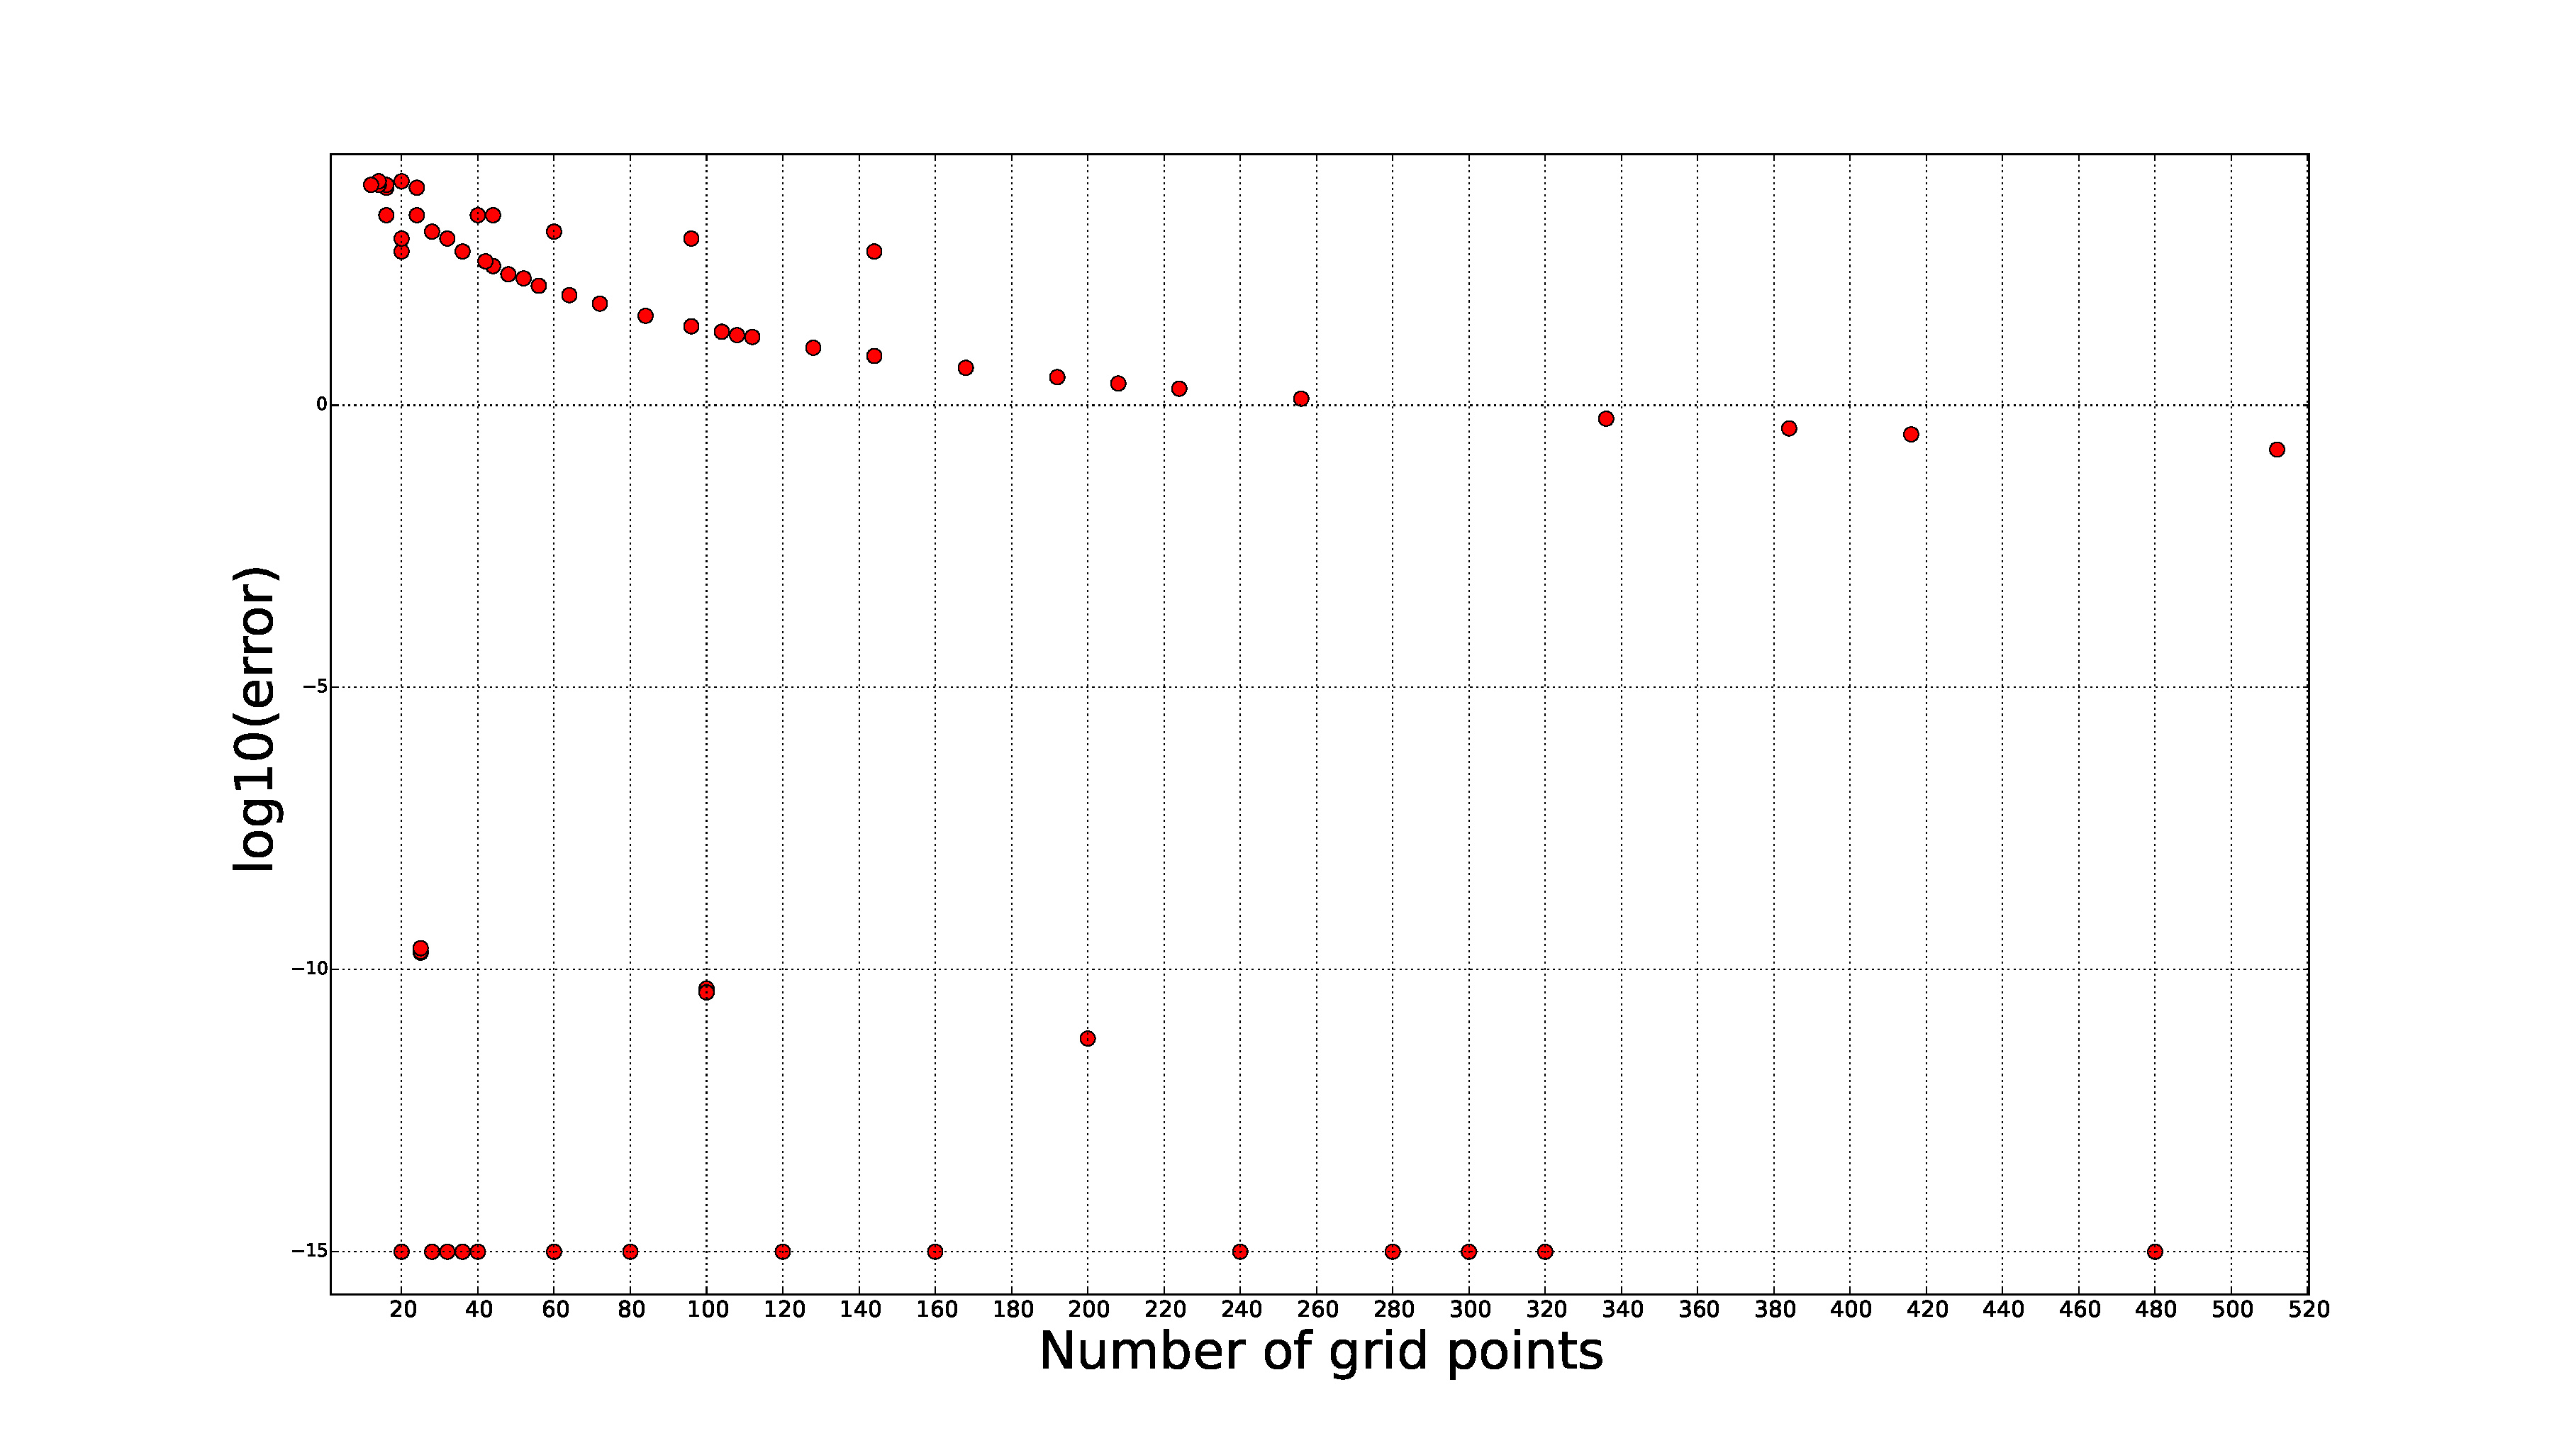
\includegraphics[scale=0.3]{gridPoints}
	    \centering 
    \caption{Error plots for different set of parameters for the PME.}    
		\label{fig:grid}   
   \end{figure}  
   
   This hypothesis has been tested in Figure (\ref{fig:grid}) : The number of grid points used for each simulation has been plotted according to the corresponding error. It can be seen that the error is very small for a number of grid points of $20,40,60,80,120,160,240,280,300,320$ which are all multiple of 20. This would explain the striped pattern seen on the error plot figure 4.7.


\section{Comparing with a random system}

	Because of artifacts seen figure 4.10. We decided to simulated a system composed of $N=1000$ randomly generated particles within a box size of 100 nm. The parameter ranges are the same as section 4.5.

	In this case we can't compare to an analytical solution, so the results have to be compared with a reference solution. In this case, I took the FMM forces with Depth=5, Multipole Order = 40 and WS = 2 as it is the FMM solution with the highest accuracy available. For each set parameters is computed the average relative error of the force compared to a reference solution.
	
	\begin{equation}
	 \langle \epsilon_r \rangle	= \frac{1}{N}| \vec{F}_{PME} - \vec{F}_{\text{reference}} |
	\end{equation}		
	
	where $|\cdot|$ is the Euclidean norm in $\mathbb{R^N}$

		    \begin{figure}[H]
  \label{fig:FMM_contour}
    \centering  
 \subfloat[Error plot for $WS=1$] { \centering   \includegraphics[scale=0.18]{random_FMM_WS1}}\\    
  \subfloat[Error plot for $WS=2$] { \centering  \includegraphics[scale=0.18]{random_FMM_WS2}}\\   
\subfloat[Error plot for $WS=3$] { \centering  \includegraphics[scale=0.18]{random_FMM_WS3}}\\    
  
  
    \caption{Error plots for different set of parameters for the FMM. The error is computed as stated in equation (\ref{eq:errorNaCl}). The plot are computed for $WS =$ 1(top), 2(middle), 3(bottom)}    
   \end{figure}  


\begin{figure}[H]
	   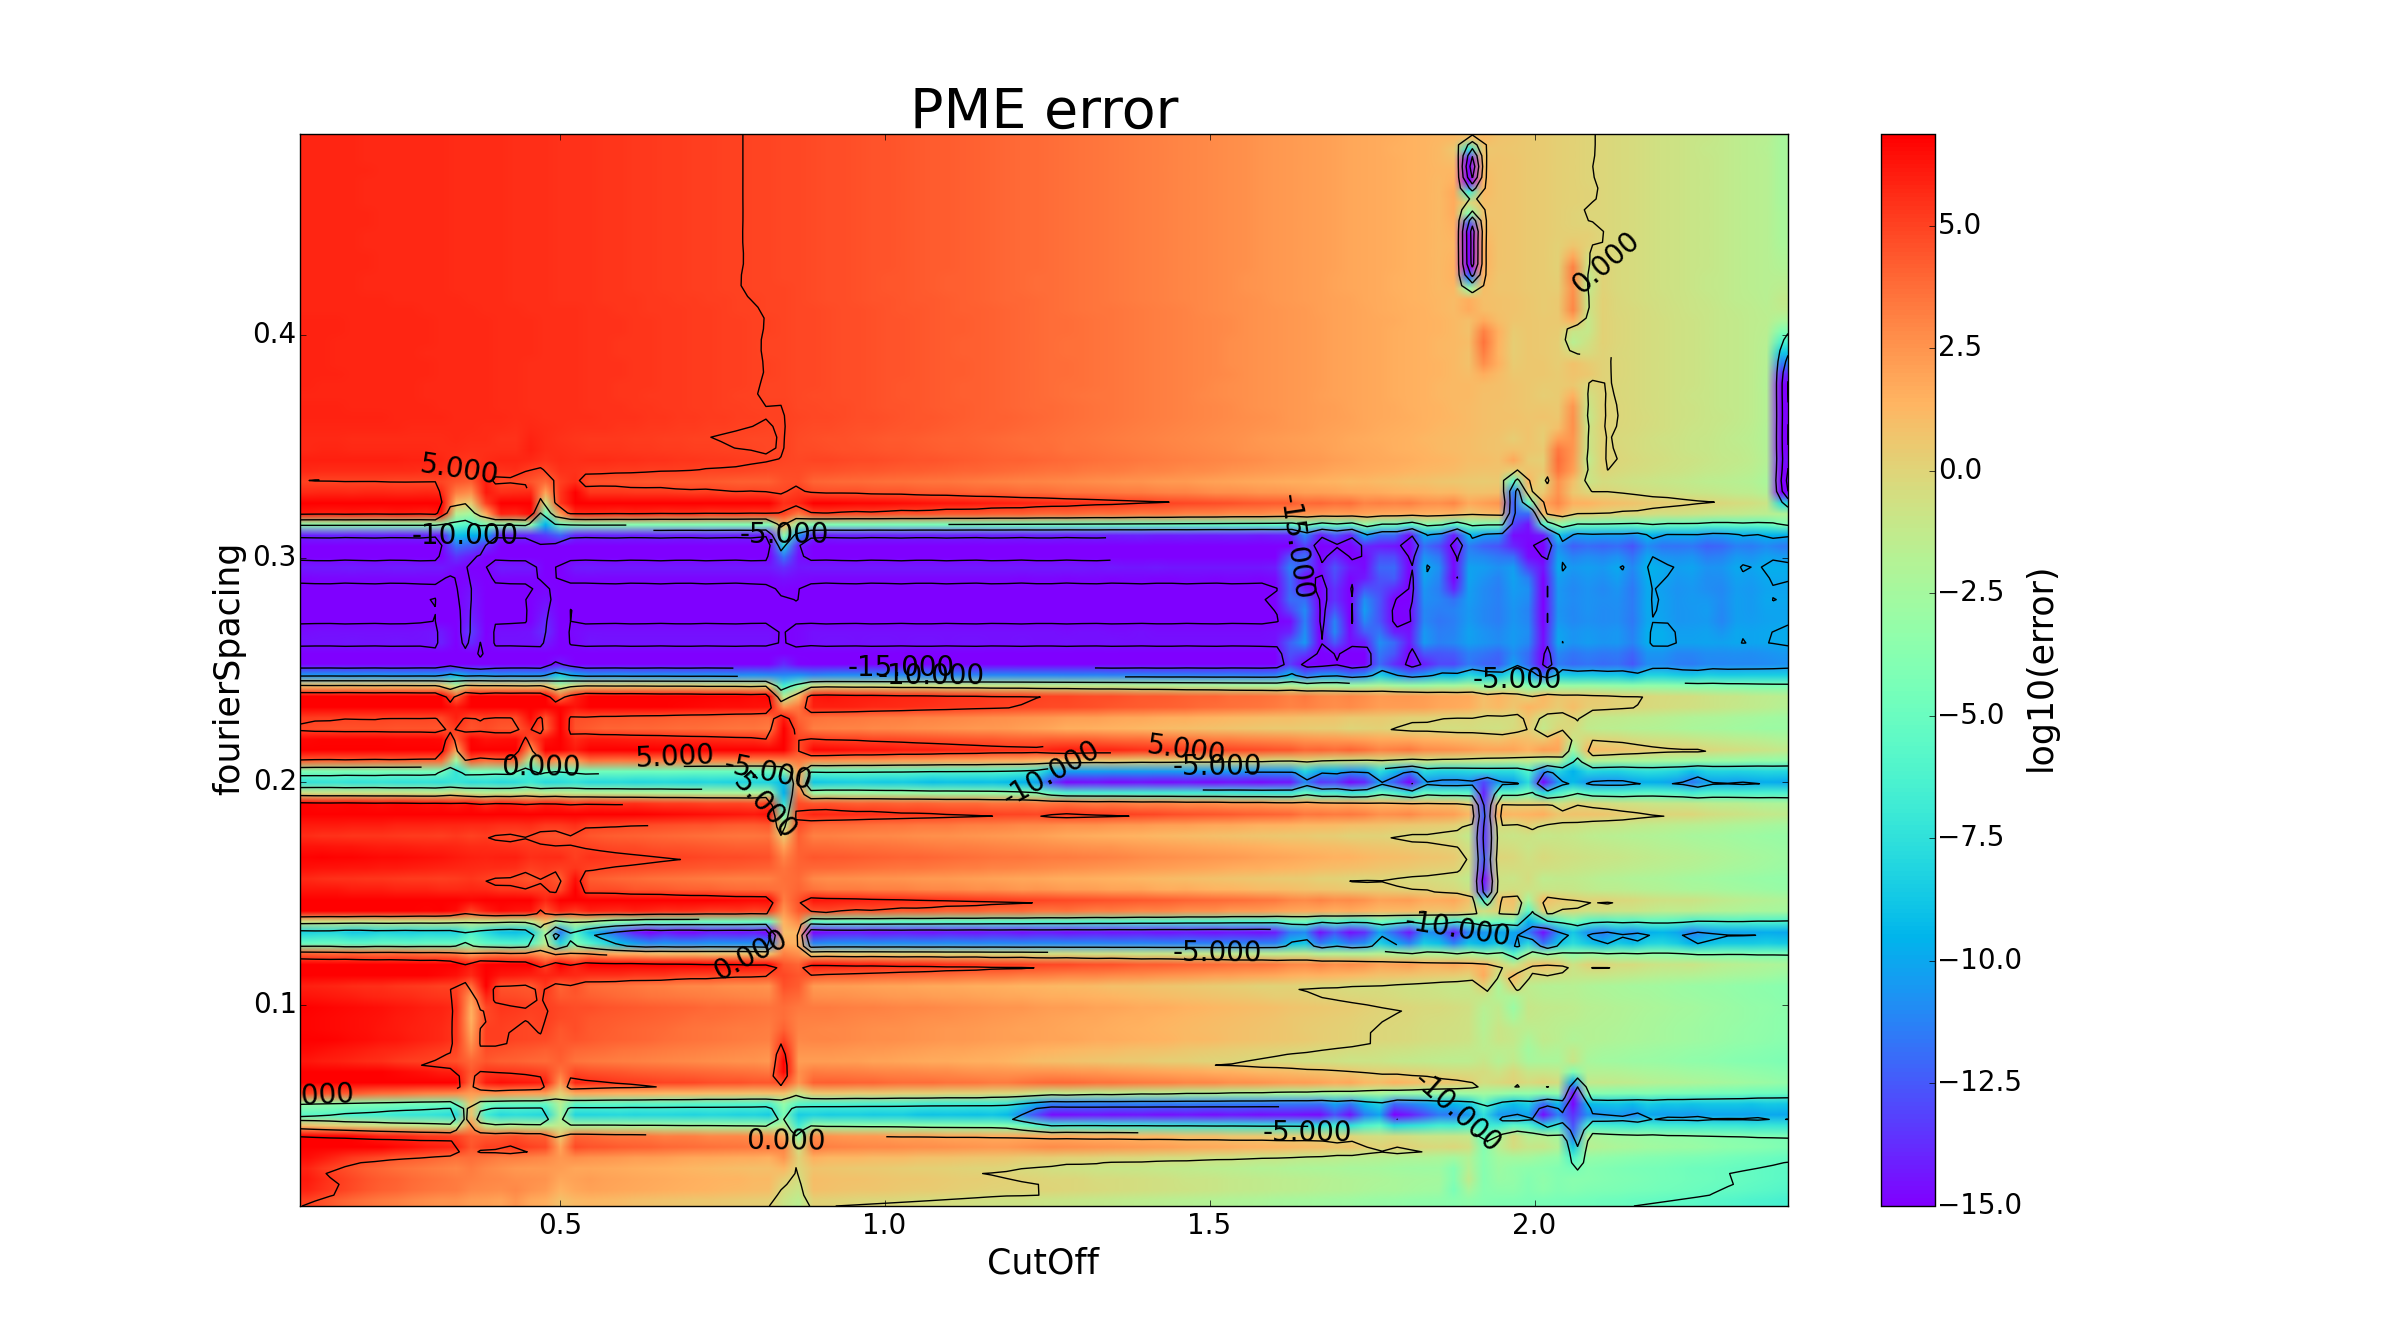
\includegraphics[scale=0.3]{PME_error}
	    \centering 
    \caption{Error plots for different set of parameters for the PME.}    
   \end{figure}

\chapter{Conclusion}

Here I conclude and finish my thesis ....
	
	
	
	

\nocite{*}
\bibliographystyle{abbrv}
\bibliography{biblio} 

\begin{appendices}
\chapter{Glossary and Abbreviations}

\begin{description}


\item[MD]  Molecular Dynamics
\item[GROMACS] GROningen MAchine for Chemical Simulations
\item[PME] Particle Mesh Ewald
\item[FMM] Fast Multipole Method
\item[Owl] MPI-BPC Cluster Used to make the Simulations

\item[MPI] Message Passing Interface
\item[OMP] OpenMP
\item[VMD] Visual Molecular dynamics


\end{description}


\chapter{Structure of Gromacs files}

\section{pdb file}

\begin{verbatim}
TITLE	Generated by qxyz2gomacs.py
REMARK	THIS IS A SIMULATION BOX
CRYST1  100.000  100.000  100.000  90.00  90.00  90.00 P 1           1
MODEL        1
ATOM      1   NA  NA     2       0.000   0.000   0.000  1.00
ATOM      2   NA  NA     4       5.000   5.000   0.000  1.00
ATOM      3   NA  NA     6       5.000   0.000   5.000  1.00
ATOM      4   NA  NA     8       0.000   5.000   5.000  1.00
ATOM      5   NA  NA    10       0.000   0.000  10.000  1.00
ATOM      6   NA  NA    12       5.000   5.000  10.000  1.00
ATOM      7   NA  NA    14       5.000   0.000  15.000  1.00
ATOM      8   NA  NA    16       0.000   5.000  15.000  1.00
ATOM      9   NA  NA    18       0.000   0.000  20.000  1.00
...
...
TER
ENDMDL
\end{verbatim}

\section{top file}


\begin{verbatim}
; topology file for a NaCl melt
;

; Include forcefield parameters
#define _FF_CHARMM
[ defaults ]
; nbfunc        comb-rule       gen-pairs       fudgeLJ fudgeQQ
1       2       yes     1.0     1.0

[ atomtypes ]
;type atnum         mass   charge ptype           sigma  epsilon
  CLA    17    35.450000    0.000  A  0.000000000000  0.00000
  SOD    11    22.989770    0.000  A  0.000000000000  0.00000


; Include topology for ions
[ moleculetype ]
; molname   nrexcl
NA      1

[ atoms ]
; id    at type     res nr  residu name at name  cg nr  charge   
1   SOD     1   NA      NA   1  1        


[ moleculetype ]
; molname   nrexcl
CL      1

[ atoms ]
; id    at type     res nr  residu name at name  cg nr  charge   
1   CLA     1   CL      CL   1  -1   


[ system ]
; Name
NaCl melt

[ molecules ]
; Compound
NA      500
CL	500 

\end{verbatim}




\section{mdp file (longe-range electrostatics part)}

\begin{verbatim}
; OPTIONS FOR ELECTROSTATICS AND VDW

; Method for doing electrostatics
coulombtype              = PME
coulomb-modifier         = Potential-shift-Verlet
rcoulomb_switch          = 0
rcoulomb                 = 0.1

; Relative dielectric constant for the medium and the reaction field
epsilon_r                = 1
epsilon-rf               = 0

; Method for doing Van der Waals
vdw-type                 = Cut-Off
vdw-modifier             = Potential-shift-Verlet

; cut-off lengths       
rvdw_switch              = 0
rvdw                     = 0.1

; Apply long range dispersion corrections for Energy and Pressure
DispCorr                 = No

; Extension of the potential lookup tables beyond the cut-off
table-extension          = 1

; Separate tables between energy group pairs
energygrp-table          = 

; Spacing for the PME/PPPM FFT grid
fourierspacing           = 0.01

; FFT grid size, when a value is 0 fourierspacing will be used
fourier-nx               = 0
fourier-ny               = 0
fourier-nz               = 0

; EWALD/PME/PPPM parameters
pme-order                = 4
ewald-rtol               = 1E-5
ewald-rtol-lj            = 0.001
lj-pme-comb-rule         = Geometric
ewald-geometry           = 3d
epsilon-surface          = 0

\end{verbatim}















\end{appendices}



























\end{document}